%%% template.tex
%%%
%%% This LaTeX source document can be used as the basis for your technical
%%% paper or abstract. Intentionally stripped of annotation, the parameters
%%% and commands should be adjusted for your particular paper - title, 
%%% author, article DOI, etc.
%%% The accompanying ``template.annotated.tex'' provides copious annotation
%%% for the commands and parameters found in the source document. (The code
%%% is identical in ``template.tex'' and ``template.annotated.tex.'')

\documentclass[annual]{acmsiggraph}

% the natbib package allows both number and author-year (Harvard)
% style referencing;
%\usepackage{natbib}

% if you use PostScript figures in your article
% use the graphics package for simple commands
% \usepackage{graphics}
% or use the graphicx package for more complicated commands
% or use the epsfig package if you prefer to use the old commands
% \usepackage{epsfig}

%\usepackage{subfigure}
%\usepackage{pstricks}
\usepackage{graphicx}
\usepackage{caption}
\usepackage{subcaption}
% The amssymb package provides various useful mathematical symbols
\usepackage{amsmath}
\usepackage{amssymb}
%\usepackage{amsfonts}
%\usepackage{mathptmx}
%\usepackage{color}
\usepackage{mathrsfs}
\usepackage{color}
%\usepackage{subfigure} %subfigure

\TOGonlineid{148}
\TOGvolume{0}
\TOGnumber{0}
\TOGarticleDOI{1111111.2222222}
\TOGprojectURL{}
\TOGvideoURL{}
\TOGdataURL{}
\TOGcodeURL{}

\title{A Sparse Shape Descriptor Using Radial Basis Function on Medial Axis}
\author{Zheng, Wenni\thanks{e-mail:wnzheng@cs.hku.hk}\\Department of Computer Science, the University of Hong Kong}
\author{Wang, Jun}
\author{Chen, Falai}
\author{Yang, Zhouwang}
\author{Wang, Wenping\thanks{e-mail:wenping@cs.hku.hk}}
\pdfauthor{Zheng, Wenni}

\keywords{convex optimization, radial basis function, medial axis, shape descriptor, sparsity}

\begin{document}

%% \teaser{
%%   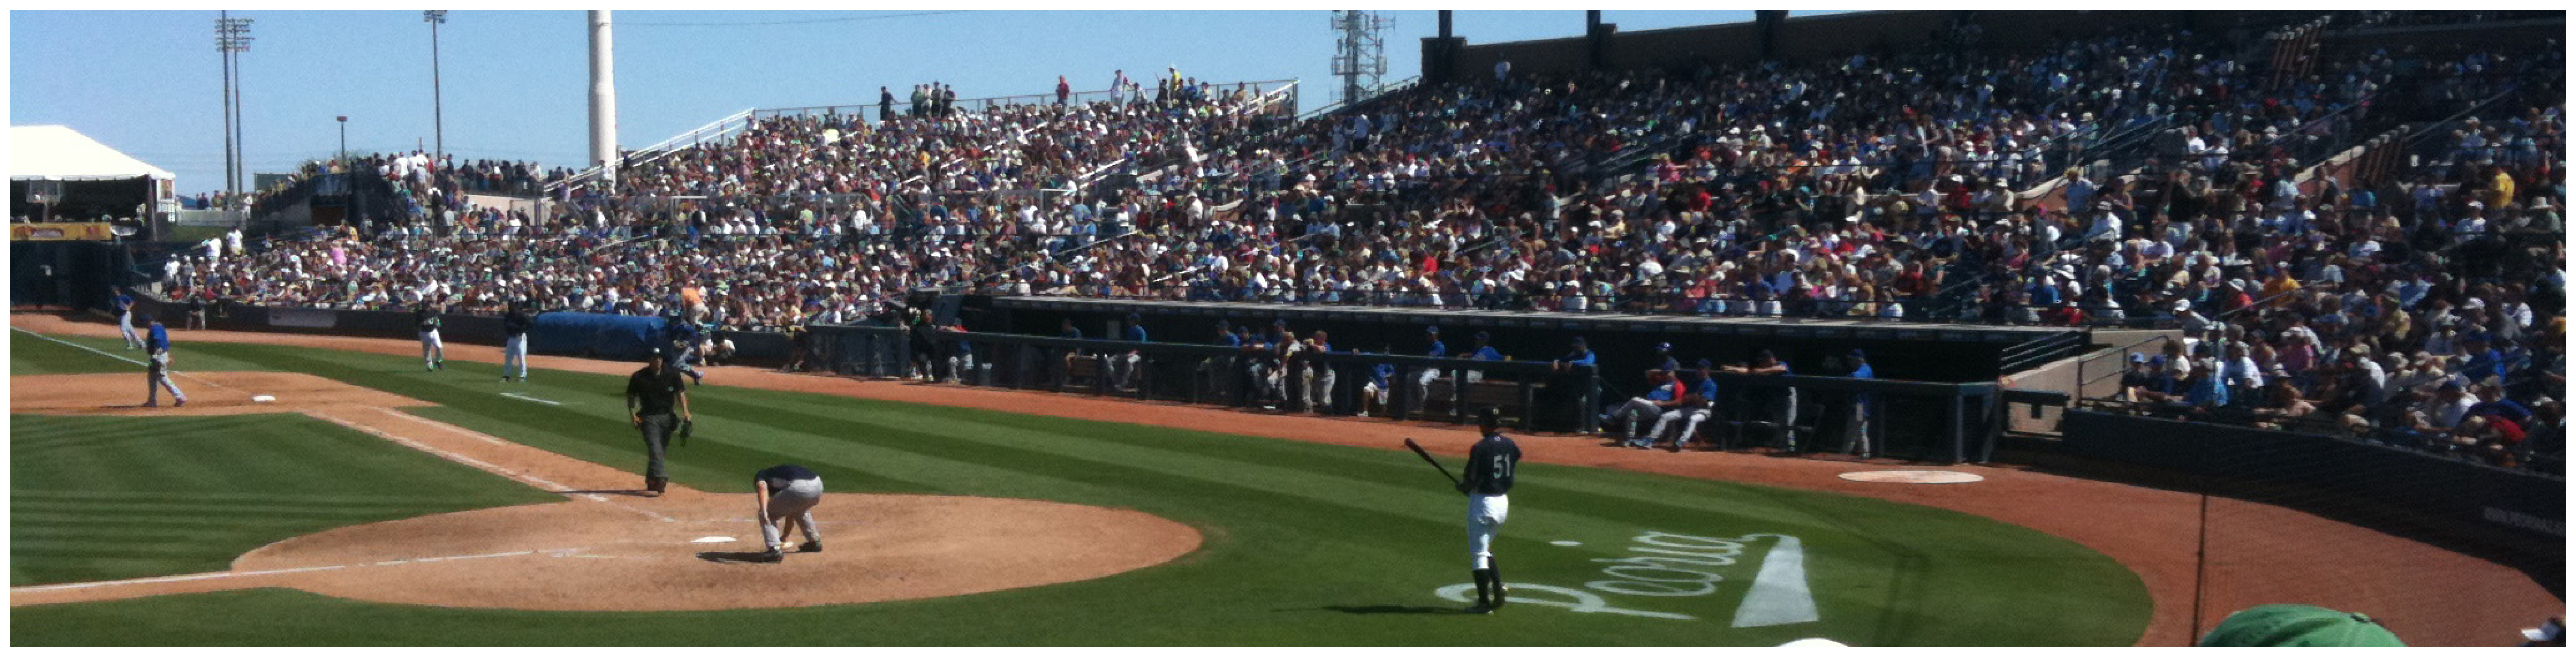
\includegraphics[height=1.5in]{images/sampleteaser}
%%   \caption{Spring Training 2009, Peoria, AZ.}
%% }

\maketitle

\begin{abstract}

%Fitting planar points is a fundamental problem in geometric modeling. In this paper, we study the fitting problem using radial basis function, and bring forward a new fitting method which has fewer variables, lighter computational load and sparser result than previous approaches. Unlike traditional methods focusing only on the shape of the fitting curve, our approach aims to build up a signed distance field from the data points as well as their medial axis. In this way, the radial basis function, which is actually served to approximate the distance field we built, will naturally reconstruct the target shape formed by the data points. Our method is packed as a convex optimization problem with $L^1$-regularization so that we could also exploit the sparsity of the solution at the same time as the minimization problem is solved. 

\end{abstract}

%\begin{CRcatlist}
%  \CRcat{I.?.?}{Computer Graphics}{SOME SUBFIELD}{Geometric Modeling}
%\end{CRcatlist}

\keywordlist

%\TOGlinkslist

\copyrightspace

\section{Introduction}



Our method targets at 3 different goals: 1) The isosurface should convinciningly describe the target shape, 2) The isosurface should not contain any extra patches which does not lay on the point cloud and 3) The isosurface should be represented by a sparse representation of radial basis function. For the first goal, we follow the tradition of using $L^2$-error to measure the quality of isosurface. Our method differs from former approaches in the second goal.

In previous literatures, to eliminate extra patches, normal information of data points is usually needed, and noise presented in normals tends to distort the reconstructed surface. With the medial axis of the shape, our method does not need any normal information. Furthermore, we observed that, as the medial axis points locate on the 'ridges' of the distance field, we could actually use the radial basis function to approximate the whole distance field inside the shape. In this way, the radial basis function will naturally reconstruct the target shape. We should note that we do not have medial axis infomation outside the shape, so it is roundless for us to reconstruct distance field outside the shape as well. Fortunately, we do not need to determine the whole distance field outside the shape in order to eliminate the extra patches of the implicit function. Instead, as described in [SECTION], we simply put some grid points outside the shape and limit the value of radial basis functions be smaller than a small negative constant value (set as $-0.01$ in this paper). These grid point constraints proved to be powerful enough to exclude all extra patches in practice.

Most of the previous methods are down-to-top approaches, focusing on reconstruction and do not intend to seek for a sparse representation of result. Medial axis, on the other hand, was well-known as a shape descriptor used for skeleton extraction, shape comparison, deformation, etc. In some sense, our method uses the combination of spheres locating on medial axis to depict the target shape, and therefore bridges the target shape and its medial axis, not through medial axis tranformation(MAT), but utilizing radial basis functions. Furthermore, it is natural to ask, in order to describe the shape within the limit of a given error bound, what is the number of radial basis needed? As it's hard to estimate the dimension of problem in the beginning, we determine to exploiting the sparisity in the radial basis function during the process of optimization. Sparsity, the number of non-zero coefficients of radial basis, is actually the $L^0$-norm of the coefficient vector. However, it well known that minimizing $L^0$-norm of a vector is NP-hard. In recent decades, substitutions of $L^0$-norm, including $L^1$-norm, weighted $L^1$-norm, are studied comprehensively in statistical learning.  In section [XXX], we will study how the distribution of initial radial basis centers affects reconstruction quality.


In sum, the optimization problem we constructed aims for the following targets:
\begin{itemize}
\item Coefficients of the radial basis' should be sparse;
\item Powerwise $L^2$-error between data points and the radial basis function is smaller than $\epsilon_1$;
\item The radial basis function should approximate the signed distance field of the input shape if possible; 
\item Value of the radial basis function stays larger than 0 inside the boudnary and smaller than 0 outside the boundary.
\end{itemize}


\section{Literature Review}


% Radial Basis Function and implicit function

\textbf{Medial Axis. }
Our method depends on medial axis information as input. Medial axis, defined as the set of points which have at least two closest neighbors on a shape, is a shape descriptor which has one-to-one correspondence to the shape through medial axis transform []. Representative algorithms designed for practical medial axis computation include the Power Crust algorithm[], [CULVER2004] and  Siddiqi et al. [2002]. Medial axis information is widely used in deformation, skeletonization, shape comparison, etc. However, the medial axis of a shape is known to be unstable: A small change on the shape may leads to significant variation of medial axis[]. To overome this drawback, various approaches contribute to improve the stability by pruning, filtering or modifying the original medial axis. Approaches by [][][] and [] evaluate the quality of medial axis points by computing the object angle formed by the medial axis point and its two cloest neighbors on the shape. Small object angle is considered as a sign of instability and the corresponding medial axis points will be filtered. The $\lambda$-medial axis by [] uses the radius of medial axis sphere to evaluate the importance of medial axis points, and medial axis spheres of small radius will be deleted. The $x$

\textbf{Implicit Function in Geometric Modeling. }

The problem of reconstructing a surface from unorganized points has long been studied in
computer graphics community and there is a lot of literature on it. Here we only review 
the closely related surface reconstruction algorithms - the implicit methods. 

The implicit methods reconstruct the surface as the zero set of a scalar function. 
The difference of these methods is on how to represent and compute the implicit function.
In ~\cite{Hoppe-etal-1992}, a signed distance field is estimated as the distance to the oriented
tangent plane of the closest point. \cite{Curless-Levoy-1996} compute the signed distance for each range
scan and blend them together to form the implicit function. \cite{Ohtake-etal-2003} propose the multi-level
partition of unity method, which hierarchically partition the data domain into sub-domains and fit data in
each sub-domain with local shape functions which are blended together using partition of unity. 
\cite{Wang-etal-2011} use the PHT-splines to approximate signed distance fields and propose a parallel and 
adaptive reconstruction algorithm.\cite{Calakli-etal-2011} present a variational approach to reconstruct a smooth signed
distance function by constraining the normals to be the gradient of signed distance functions.
Radial basis functions(RBFs)~\cite{Savchenko-etal-1995} are one class of powerful functions which are commonly used in surface reconstruction.
In~\cite{Turk-O'Brien-1999,Carr-etal-2001,Dinh-etal-2002,Turk-OBrien-2002}, the implicit RBF is constructed by placing zero function value
at each point and non-zero constraints at the offset-surface points. However, since the global RBFs have global support, 
these methods should solve a linear dense and ill-conditioned system. ~\cite{Morse-etal-2001,Kojekine-etal-2003,Ohtake-etal-2003b} employ 
compactly supported RBFs to reduce computation cost and speed up reconstruction. Instead of putting centers of the RBFs'
basis function on the data points, \cite{Samozino-etal-2006} put them on the medial axis and use radius of the corresponding medial axis point
to compute the local support size. Moreover, \cite{Submuth-etal-2010} alternatingly optimize the weights of the RBFs and the positions of the RBFs centers in the RBFs based reconstruction.

Besides signed distance functions, indicator functions are recently used in surface reconstruction. Points equipped with oriented
normals are viewed as samples of the gradient of an indicator function~\cite{Kazhdan-etal-2005,Kazhdan-etal-2006,Manson-etal-2008,Kazhdan-etal-2013}.
In~\cite{Kazhdan-etal-2005}, Fourier series are used to represent indicator functions in a uniform grid. 
The Fourier series approach is then improved by poisson reconstruction ~\cite{Kazhdan-etal-2006}, which adopts hierarchical locally supported 
functions and compute the indicator function by solving a Poisson problem. In~\cite{Manson-etal-2008}, wavelets are used
to represent the indicator function and a streaming surface reconstruction algorithm is proposed. \cite{Kazhdan-etal-2013} propose the
screened poisson reconstruction, extending poisson reconstruction by explicitly incorporating the points as interpolation constraints.

\textbf{Sparsity in Geometry Representation. } 

\textbf{Convex Optimization Algorithms. }
Our method will solve an constrained $L^1$-norm regularized minimization problem. Algorithms for this type of problem are intensively studied in literatures of statistics and machine learning. Most notable algorithms include the classic Least Angles Regression(LARS), the Bregman iterative algorithm, the interior point method and its variation implemented in the CVX solver, gradient projection methods, etc. Most of these algorithms have unique advantages and suitabilities. Since our problem will deal with a large number of variables and constraints, the capacity to solve large scale problems is priorized when choosing different algorithms. The Alternating Direction Method of Multipliers (ADMM) is an algorithm based on the Augmented Lagrangian Method. Unlike many previous approaches which construct large linear system from the mixture of objective function and constraints, ADMM provides a scheme to split variables in the Lagragian. Consequently, the original large scale problem will be decomposed into a group of smaller problems, and these small problems will be solved in a sequential manner in every iteration. Therefore, ADMM is well adapted to solve large scale constrained convex problems. Literature [][] gives comprehensive introduction to ADMM, while [] [] and [] are representive publications focusing on convergence speed and parameter selection of ADMM.

\section{Methods}

This section introduces details our method: Data points and medial axis as input, then the definition of the radial basis function we used. After that, two types of optimization constraints are explained. After that, we discuss the solver used for the convex optimization problem and sparsity for the final result. A planar example is provided in Figure [] as a flowchart to illustrate our method. 

\textbf{Data Points. }
The input of our method is a set of data points $\{\mathbf{X}_k\}_{k=1}^N$ representing the shape of an geometric object. For uniformity, we scale all data points to the unit box $[-1,1]\times[-1,1]\times[-1,1]$. 

\textbf{Medial Axis. }
Next, we compute the medial axis of input data $\{\mathbf{X}_k\}_{k=1}^N$ by the power crust algorithm[]. The centers of these medial axis spheres are denoted as $\{\mathbf{M}_i\}_{i=1}^n$. Sphere radius corresponding to these medial axis spheres are denoted as $\{r_i\}_{i=1}^n$. We improve the statbility of medial axis by evaluting the \textit{object angle} of each medial axis sphere[]: Medial axis spheres with object angle larger than 0.8 will be removed. The remaining medial axis sphere centers and radius, still denoted as $\{\mathbf{M}_i\}_{i=1}^n$ and $\{r_i\}_{i=1}^n$ hereafter, will be used to construct the radial basis function.

\textbf{the Radial Basis Function. }
The radial basis function we used is defined as:
\begin{equation}
F(\mathbf{X})=\sum_{i=1}^nc_i\cdot B_i(\mathbf{X})+p(\mathbf{X}).
\end{equation}
Where:
1)  $B_i(\mathbf{X})$ is the i-th radial basis. We put a radial basis on every medial axis sphere center. i.e, the number of radial basis is equal to the number of medial points as input. The radial basis are chosen as Gaussian functions, which radius equal to the radius of the corresponding medial spheres:
\begin{equation}
B_i(\mathbf{X})=e^{-\frac{\|\mathbf{X}-M_i\|^2}{r_i^2}}.
\end{equation}
The definition of our radial basis differs in two aspects from the traditional approach in []: First, we center the radial basis on the center of the medial sphere, not on data points. Second, the radius of exponent term $r_i$ in the Gaussian function equals to the radius of the medial sphere. These settings allow our method to exploit the symmetry of shape brought by the medial axis information, and grant our method the adaptivity to represent multiscale shapes. The second advantage will be further explained and illustrated in the coming texts.

2) $\{c_i\}_{i=1}^n $  are coefficients of radial basis subjected to optimization.

3) $p(\mathbf{X})$ is a degree 2 polynomial, which is the same as polynomial used in []. For 3D examples, $p(\mathbf{X})$ contains 10 terms: $p(\mathbf{X})=c_{n+1}\mathbf{X}_1^2+c_{n+2}\mathbf{X}_2^2+c_{n+3}\mathbf{X}_3^3+c_{n+4}\mathbf{X}_1\mathbf{X}_2+c_{n+5}\mathbf{X}_1\mathbf{X}_3+
c_{n+6}\mathbf{X}_2\mathbf{X}_3+c_{n+7}\mathbf{X}_1+c_{n+8}\mathbf{X}_2+c_{n+9}\mathbf{X}_3+c_{n+10}.$ For 2D examples, $p(\mathbf{X})$ is a polynomial of 6 terms. The rationale of using a polynomial term in the radial basis function could be found in literatures such as [] and [].

We will use isosurface at $F(\mathbf{X})=0$ to represent the target shape. The error of the radial basis function at $\mathbf{X}_k$ is hence $|F(\mathbf{X_k})|$. We use the pointwise $L^2$-norm to evalute the reconstruction accuracy on the input data: $\sqrt{\sum_{i=1}^N F^2(\mathbf{X}_k)/N}$. 

\textbf{Distance Field within the Shape. }
Most of former reconstruction methods using implicit functions need the information of surface normal to construct a signed distance field near the target surface. These methods lack sufficient information to reconstruct the signed distance field deep inside the shape. However, with the help of medial axis this could be done : For the signed distance field built upon the input data points, suppose that we travel from a data point and climb along its gradient, then the location of the medial axis sphere center corresponding to this data point is just on the 'ridges' of distance field, which is the furthest point we could reach. Furthermore, the radius of medial axis sphere equals to the height of the distance field at the medial axis sphere center. Therefore, the location of medial axis sphere centers along with their radius actually points out the location of all 'ridges' of the distance field. Based on this fact, our method try to reconstruct the complete signed distance field within the target shape with radial basis function. Upon the completion of this goal, the isosurface at $F(\mathbf{X})=0$ of the radial basis function will naturally represent the target shape.

\textbf{Ridge Anchor Constraints. }
For a medial axis sphere centering at $\mathbf{M}_i$ with radius $r_i$, the height of the signed distance field at $\mathbf{M}_i$ should equal to $r_i$. To reconstruct the signed distance field, $F(\mathbf{M}_i)$ should not be too far way from $r_i$. We name the medial points $\{\mathbf{M}_i\}$ as 'ridge anchors' because they lay on the ridge of the signed distance field. 

We follow two principles when formulating constraints on ridge anchors: 1) Constraint on each ridge anchor should exert independently, regardless of the effectiveness of constraints on other ridge anchors. Therefore, we use $L^{\infty}$-norm instead of pointwise $L^2$-norm to evaluate error. By doing so, we prevent the situation that the radial basis function well approximates the signed distance field on most of the medial points but apparently deviates from the signed distance field on a few points of the ridge. 2) We notice that many real world shapes contain bulky parts and subtle parts simultaneously, which means the radius of different medial spheres are of different scale. Therefore, it is reasonable to use relative error instead of absolute error to evalute the approximation quality. The relative error at point $\mathbf{M}_i$ could be expressed as $|F(\mathbf{M_i})-r_i|/r_i$. It is the percentage of error relating to target height $r_i$.

\textbf{Constraints Outside the Shape. }
Now we consider the target shape of the radial basis function outside the shape. Note that in some literatures(e.g., [SGP2006]), medial spheres centered outside the shape are considered as medial axis and used for computation as well the medial spheres inside the shape. Our experience, however, shows that the medial spheres outside the shape are much more sparse than those inside the shape and, as a consequence, these medial spheres are incapable to depict the complete distance field outside (Please refer to Figure []). Based on this observation, we do not try to construct distance field outside the shape as we did inside the shape. Instead, we just require the radial basis function to be less than 0 outside. This will ensure that the isosurface at $F(\mathbf{X})=0$ will represent, and only represent the target shape, and no extra patches will appear. 

\textbf{Sign Anchor Constraints. }
We place two layers of grid points outside the shape as indicators of sign for the radial basis function: The first layer of grid points is dense and locates near the input shape, while the second layer of grid points is sparser and locates far from the shape. We require the radial basis function keeping negative value on all of these grid points. We name these grid points as \textit{sign anchors} and denote them as $\{\mathbf{G}_i\}$ in optimization. The rationale of setting two layers of grid points as constraints is: For a point near the shape, the value of the radial basis function is determined by some radial basis as well as the polynomial term. Depending on coefficients of the radial basis function, there may exist some local minimum and maximum near this point. If the grid points are not dense enough, a local maximum just larger than 0 could appear without being constrained by any of the grid points. On the other hand, for a point far away from the data points, the Gaussian function will degenerate to almost 0 and the value of the radial basis function is determined exclusively by polynomial terms, which could be regularized to be negative with much fewer constraints. In this paper, inner grid points are sampled from 50$\times$50$\times$50 grid and outer grid points are sampled from 10$\times$10$\times$10 grid. We use inner grid points when distance to nearest data point is smaller than 0.03. An illustration of two-layer grid points is presented in Figure [].

In optimization practice, we use the less-and-equal-than constraint $F(\mathbf{G}_i)\le\epsilon$ and set $\epsilon$ as a small negative constant on all grid points $\{\mathbf{G}_i\}$.

\textbf{the Convex Optimization. } Now we have summarized the constraints of the optimization problem: Pointwise $L^2$-norm constraints depicting reconstruction error, ridge anchor constraints for approximating signed distance field, and sign anchor constraints for keeping the radial basis function negative outside the shape. The final target of the optimization is to keep the sparsity of the solution. This is achieved by minimizing the $L^1$-norm of the coefficients $\{c_i\}$. To sum up, the optimization problem is formulated as:
\begin{align}
&\min\sum_{i=1}^n|c_i|,\label{eq:1}\\
s.t. &\sum_{k=1}^N F^2(\mathbf{X}_k)<\epsilon_1\cdot N^{\frac{1}{2}},\label{eq:2}\\
&\|D\cdot(F(\mathbf{M}_i)-r_i)\|_{\infty}<\epsilon_2,\label{eq:3}\\
& F(\mathbf{G}_i) \le \epsilon_3, \quad\forall \mathbf{G}_i.\label{eq:4}
\end{align}
in which $D=diag\{1/r_1,...,1/r_n\}$.

As we have explained, $\epsilon_1$ is the pointwise $L^2$-norm tolerance. $\epsilon_2$ is the percentage of error tolerance for ridge anchors. We set $\epsilon_2=20\%$ in this paper unless specified. $\epsilon_3$ is a small value used to signify negative value outside the shape. We set $\epsilon_3=-0.01$ in this paper.

\textbf{ADMM. }
We use the Alternating Direction Method of Multipliers(ADMM) to solve the above optimization problem. Briefly speaking, ADMM is an improved augmented Lagragian method which separates variables and decomposes the large Lagragian into small problems. Our optimization problem is re-organized into a problem of 9 different variables and these variables are updated one by one in every iteration. Mathematical deduction of variable updating formula and implementation details are included in Appendix [].

\textbf{Sparsity. }
Since we solve an $L^1$-regularized optimization instead of $L^0$-regularized problem, the result of ADMM may contain some small but nonzero coefficients. In the last step of our algorithm, we set the coefficients whose absolute value are smaller than $10^{-4}$ as 0. After this step, we get the final sparse representation of the radial basis function.

\section{Results and Discussions}
~\cite{Chen:2009:ABF}


\textbf{Error Bounded Sparse Representation with Medial Axis. }
Medial axis simplification problem is studied in many former literatures. However, previous work didn't tell us how the process of simplification links with the error introduced to the simplified shape comparing with the original shape. Consequently, users may feel hard to control the quality of the shape when trying to obtain a clean medial axis. Our method addresses this problem: Given an error bound $\epsilon_1$ in constraints [], our method will give a sparse representation of radial basis function, which is a linear combination of Gaussian function on some selected medial axis points. $\epsilon_1$. 
\begin{figure*}
        \centering
		\begin{subfigure}[b]{0.24\linewidth}
                \centering
                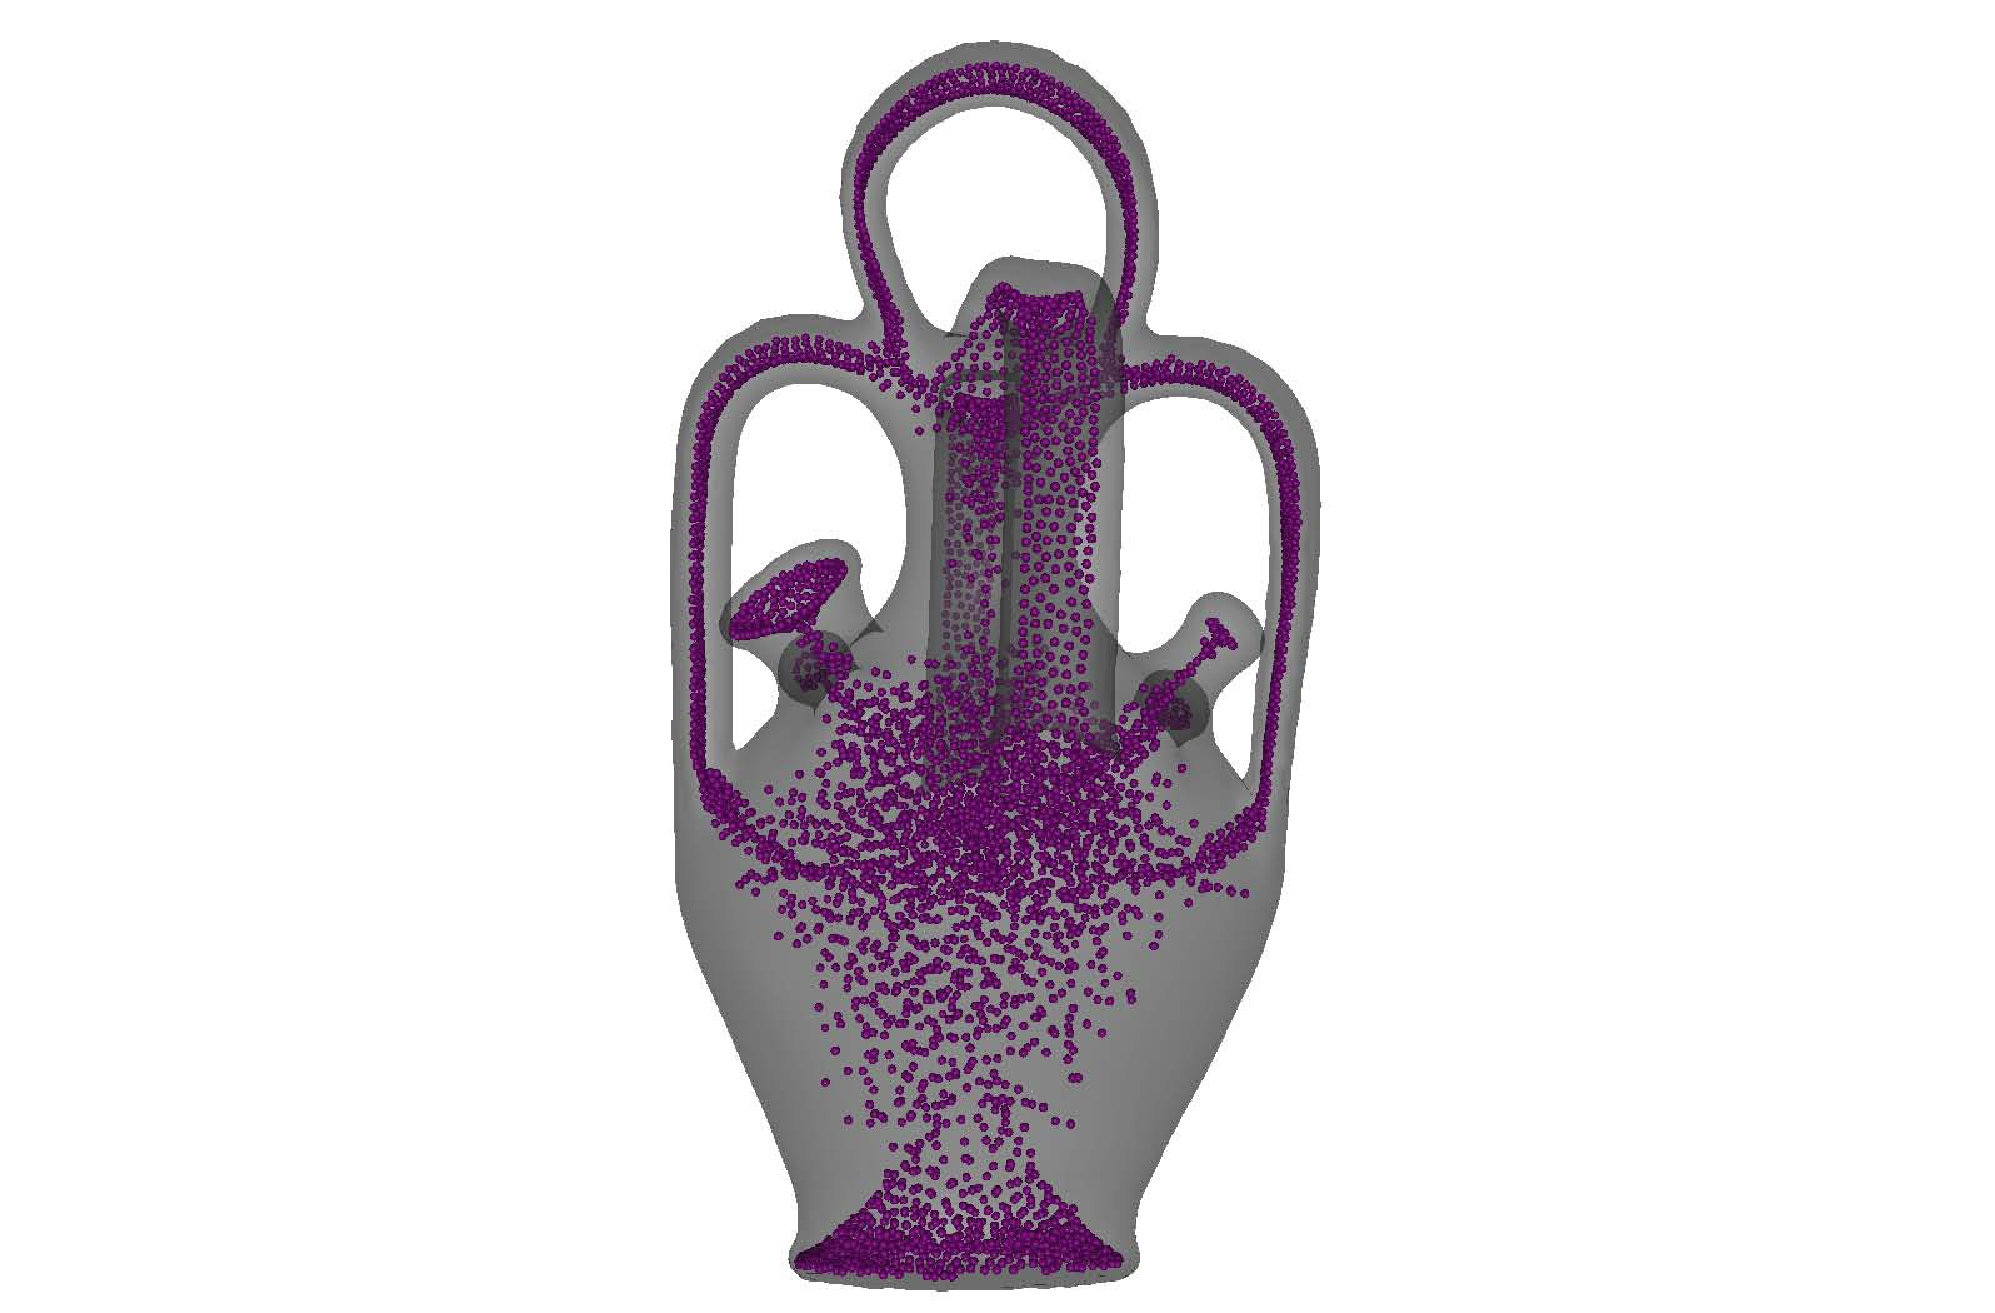
\includegraphics[width=\textwidth]{images/vase/0.pdf}
       \end{subfigure}
		~
		\begin{subfigure}[b]{0.24\linewidth}
                \centering
                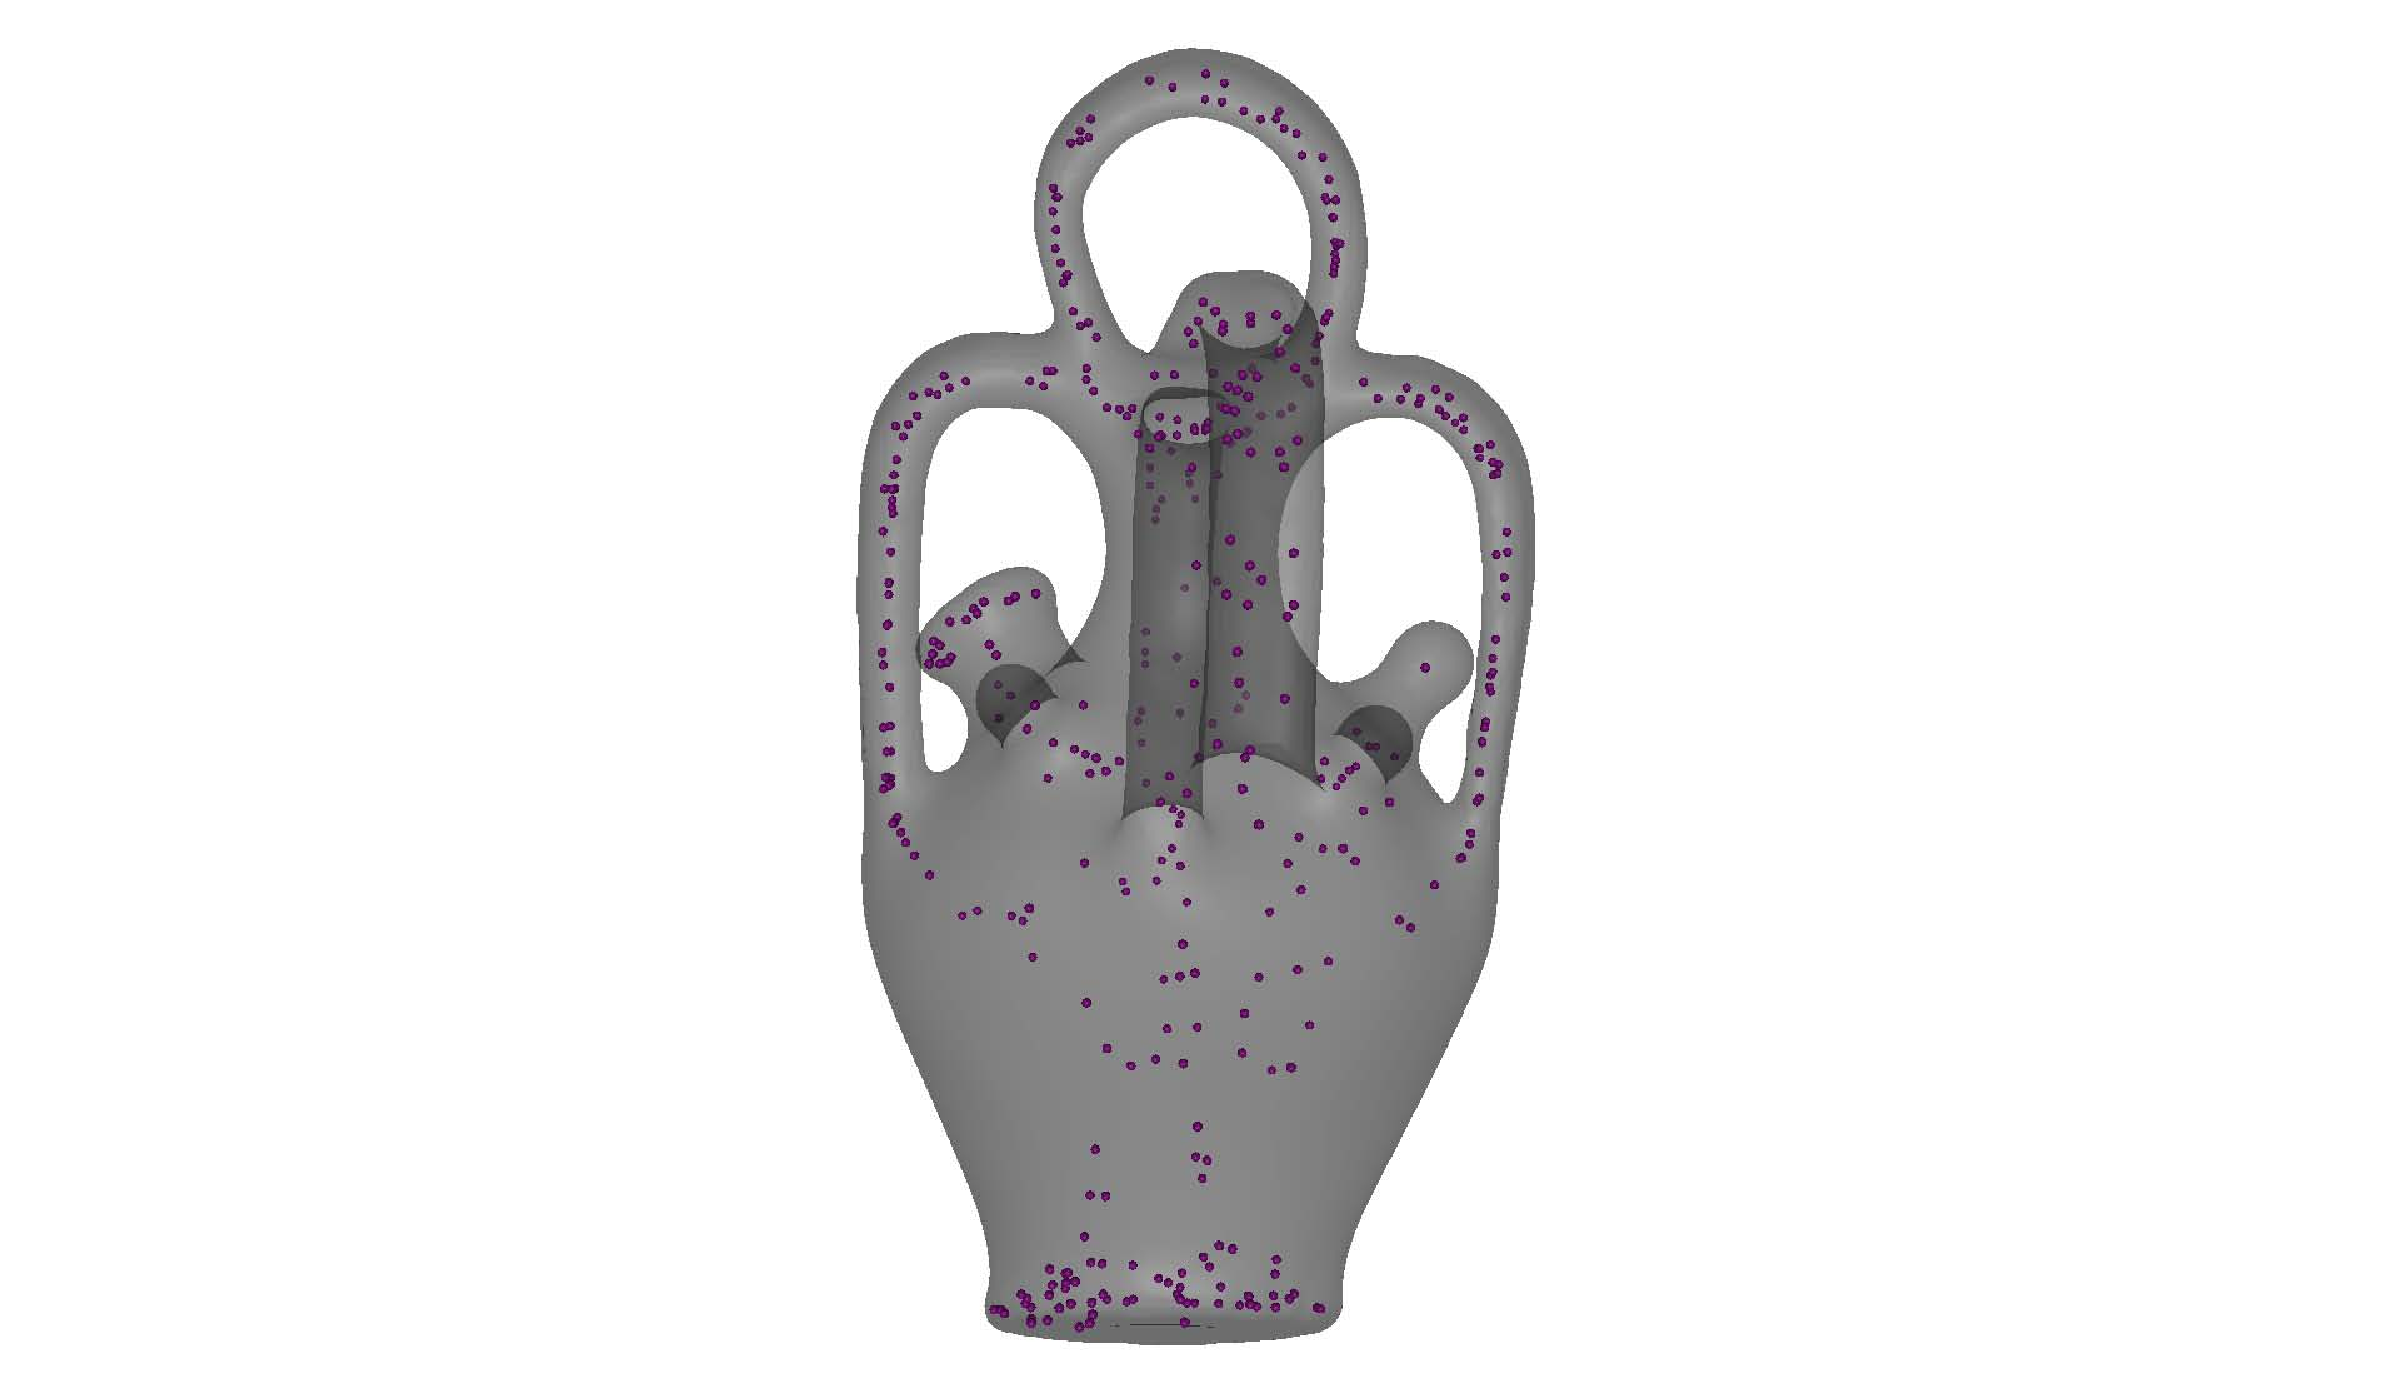
\includegraphics[width=0.92\textwidth]{images/vase/2.pdf}
        \end{subfigure}
~
		\begin{subfigure}[b]{0.24\linewidth}
                \centering
                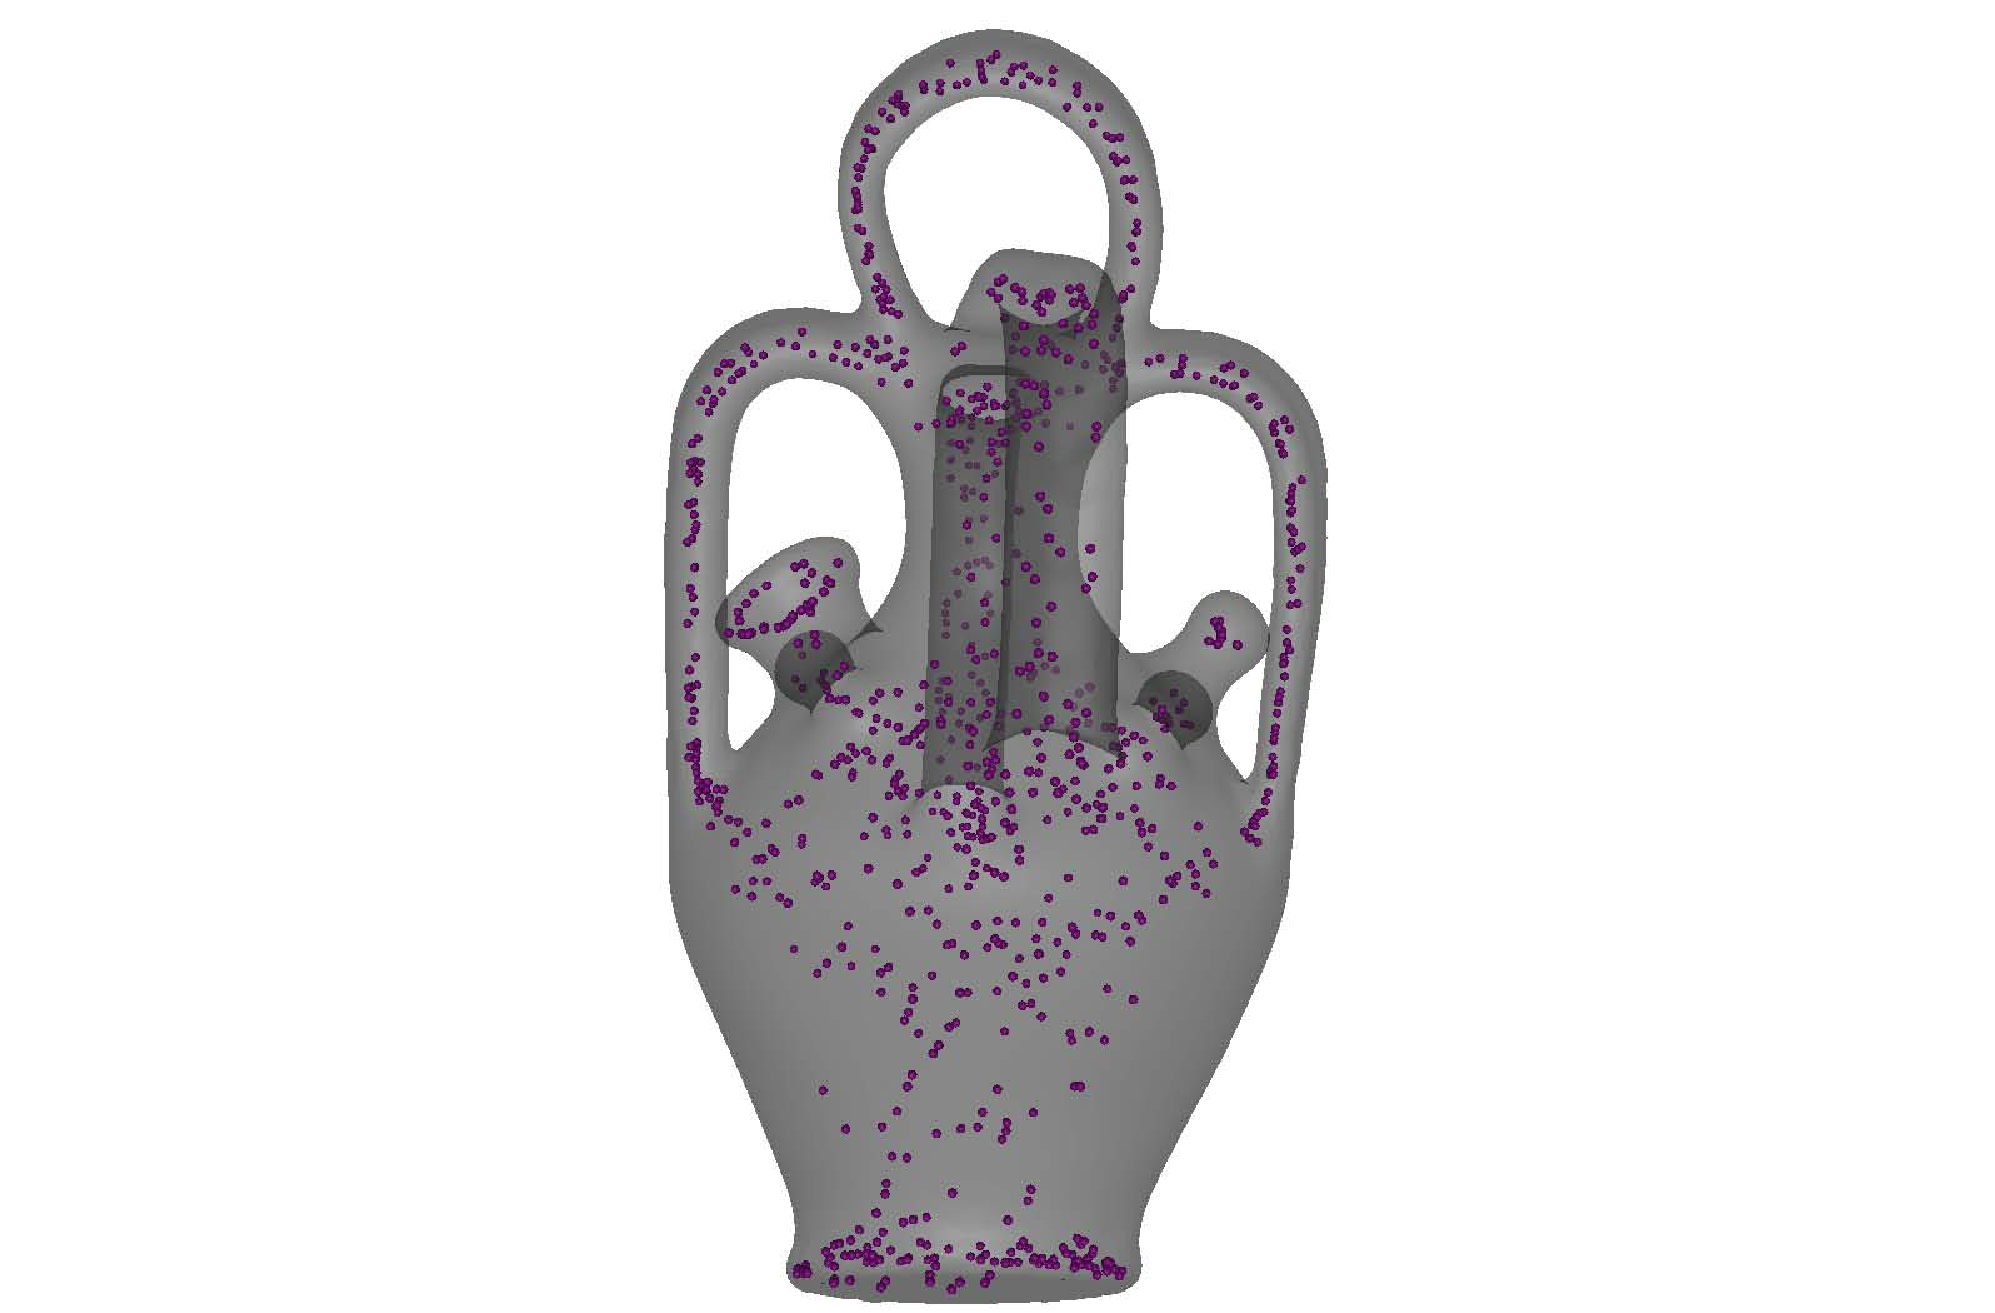
\includegraphics[width=0.98\textwidth]{images/vase/3.pdf}
        \end{subfigure}
~
		\begin{subfigure}[b]{0.24\linewidth}
                \centering
                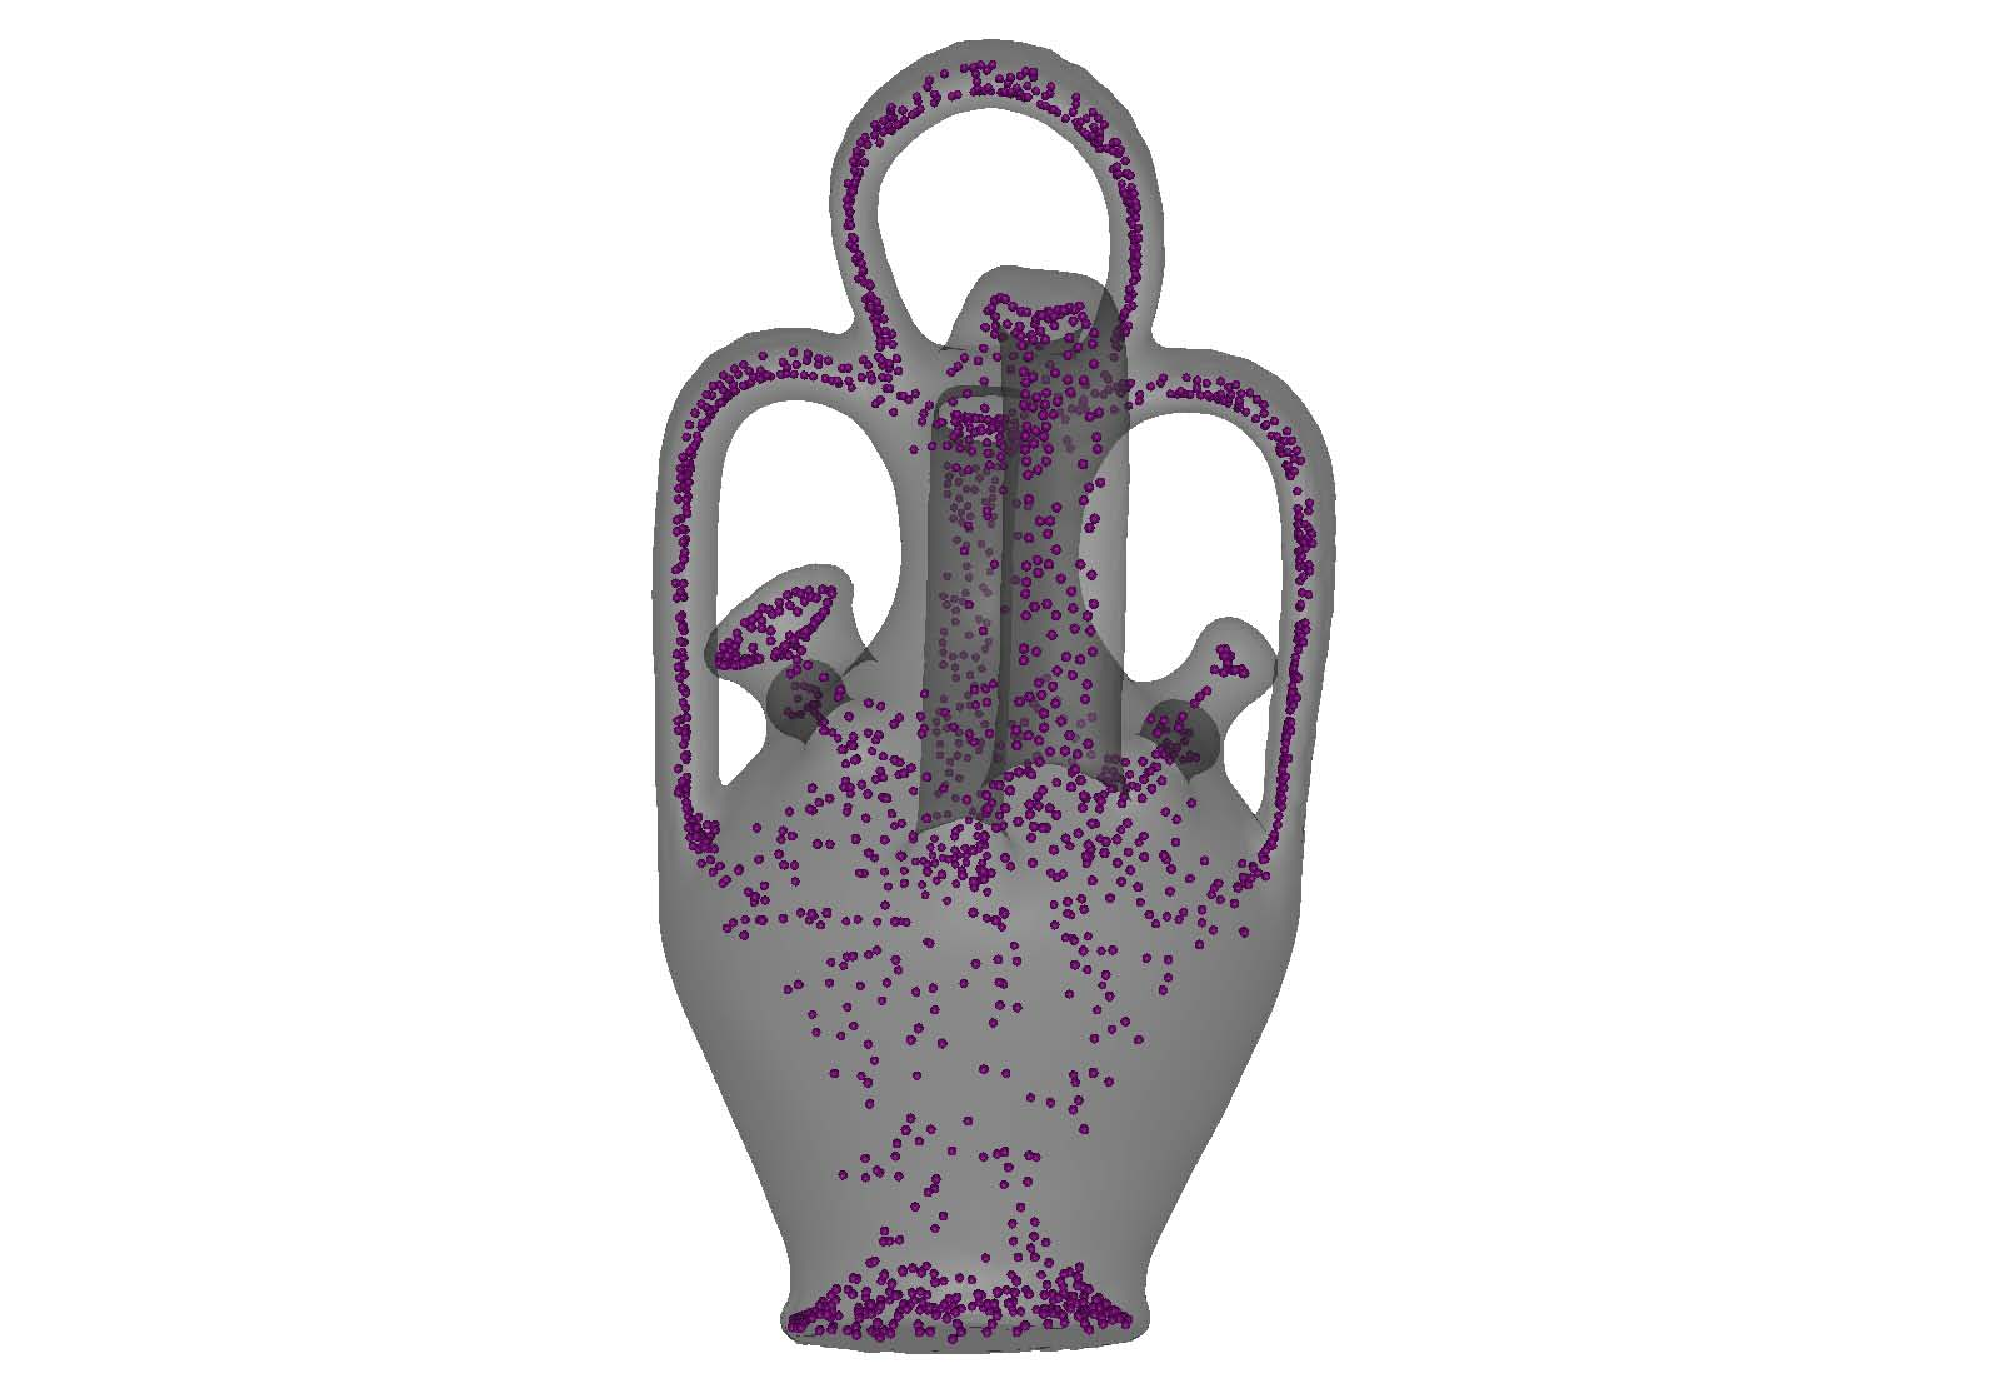
\includegraphics[width=0.92\textwidth]{images/vase/4.pdf}
        \end{subfigure}
        \caption{Chinese calligraphy which means 'horse'. From left to right: ground truth, shape of the signed distance field approximated by the radial basis function, signed distance field at height = $0.025$, $0.05$ and $0.075$, respectively. }
				\label{fig:horse}
\end{figure*}

\begin{figure*}
        \centering
		\begin{subfigure}[b]{0.19\linewidth}
                \centering
                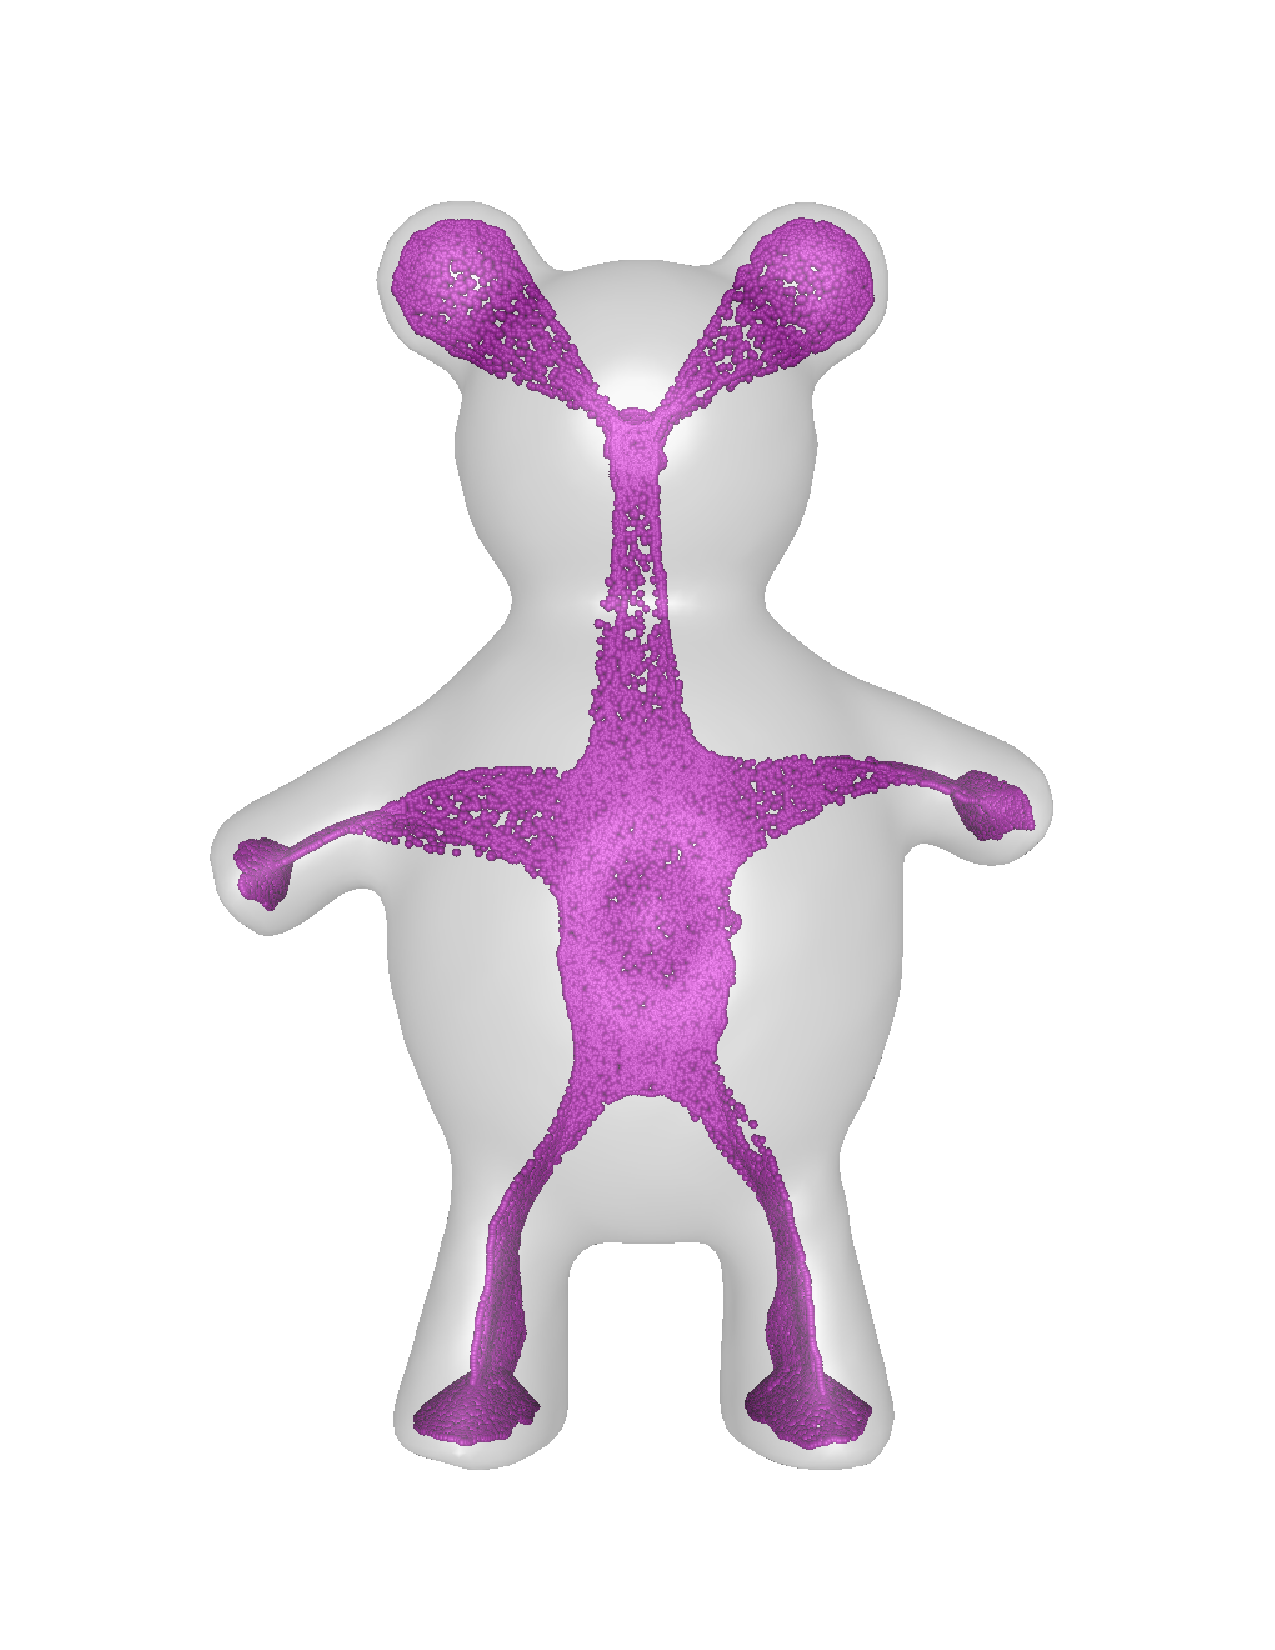
\includegraphics[width=\textwidth]{images/bear/0.pdf}
       \end{subfigure}
		~
		\begin{subfigure}[b]{0.19\linewidth}
                \centering
                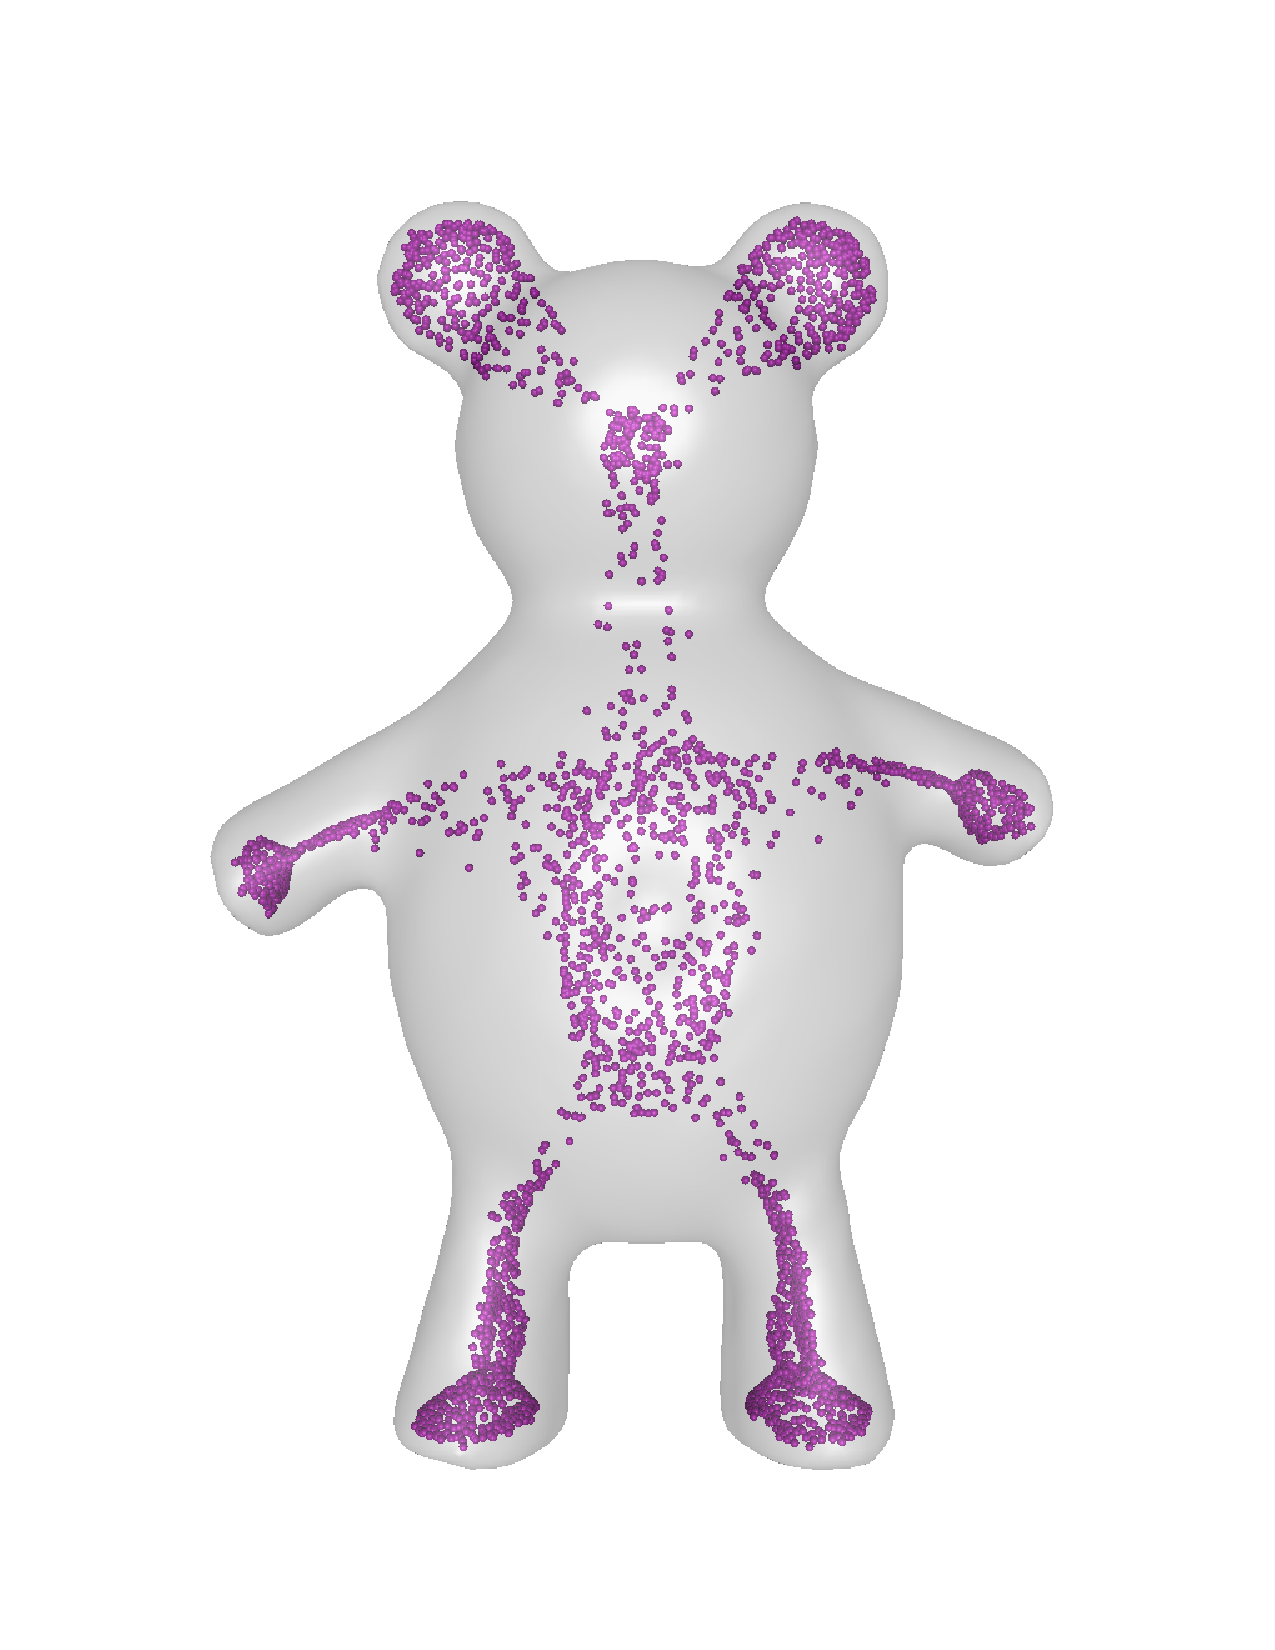
\includegraphics[width=\textwidth]{images/bear/1.pdf}
        \end{subfigure}
~
		\begin{subfigure}[b]{0.19\linewidth}
                \centering
                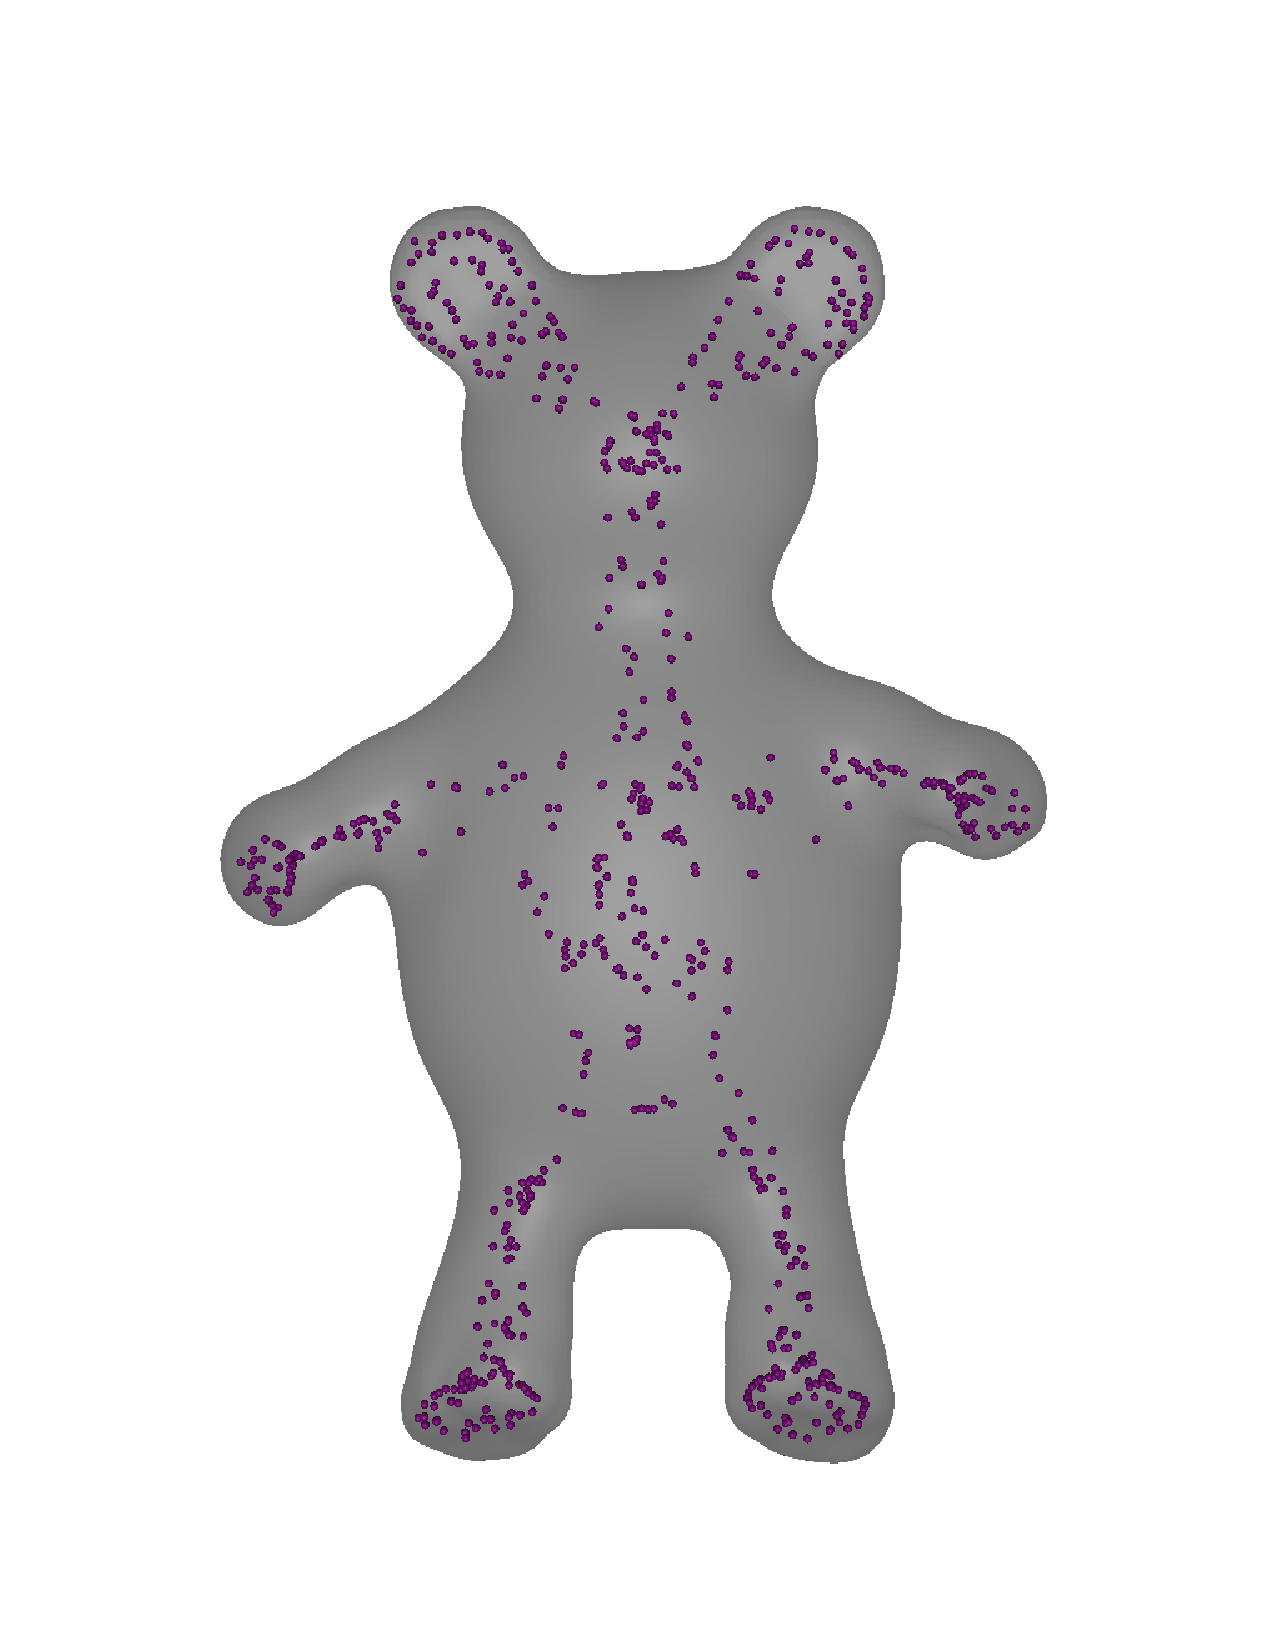
\includegraphics[width=\textwidth]{images/bear/2.pdf}
        \end{subfigure}
~
		\begin{subfigure}[b]{0.19\linewidth}
                \centering
                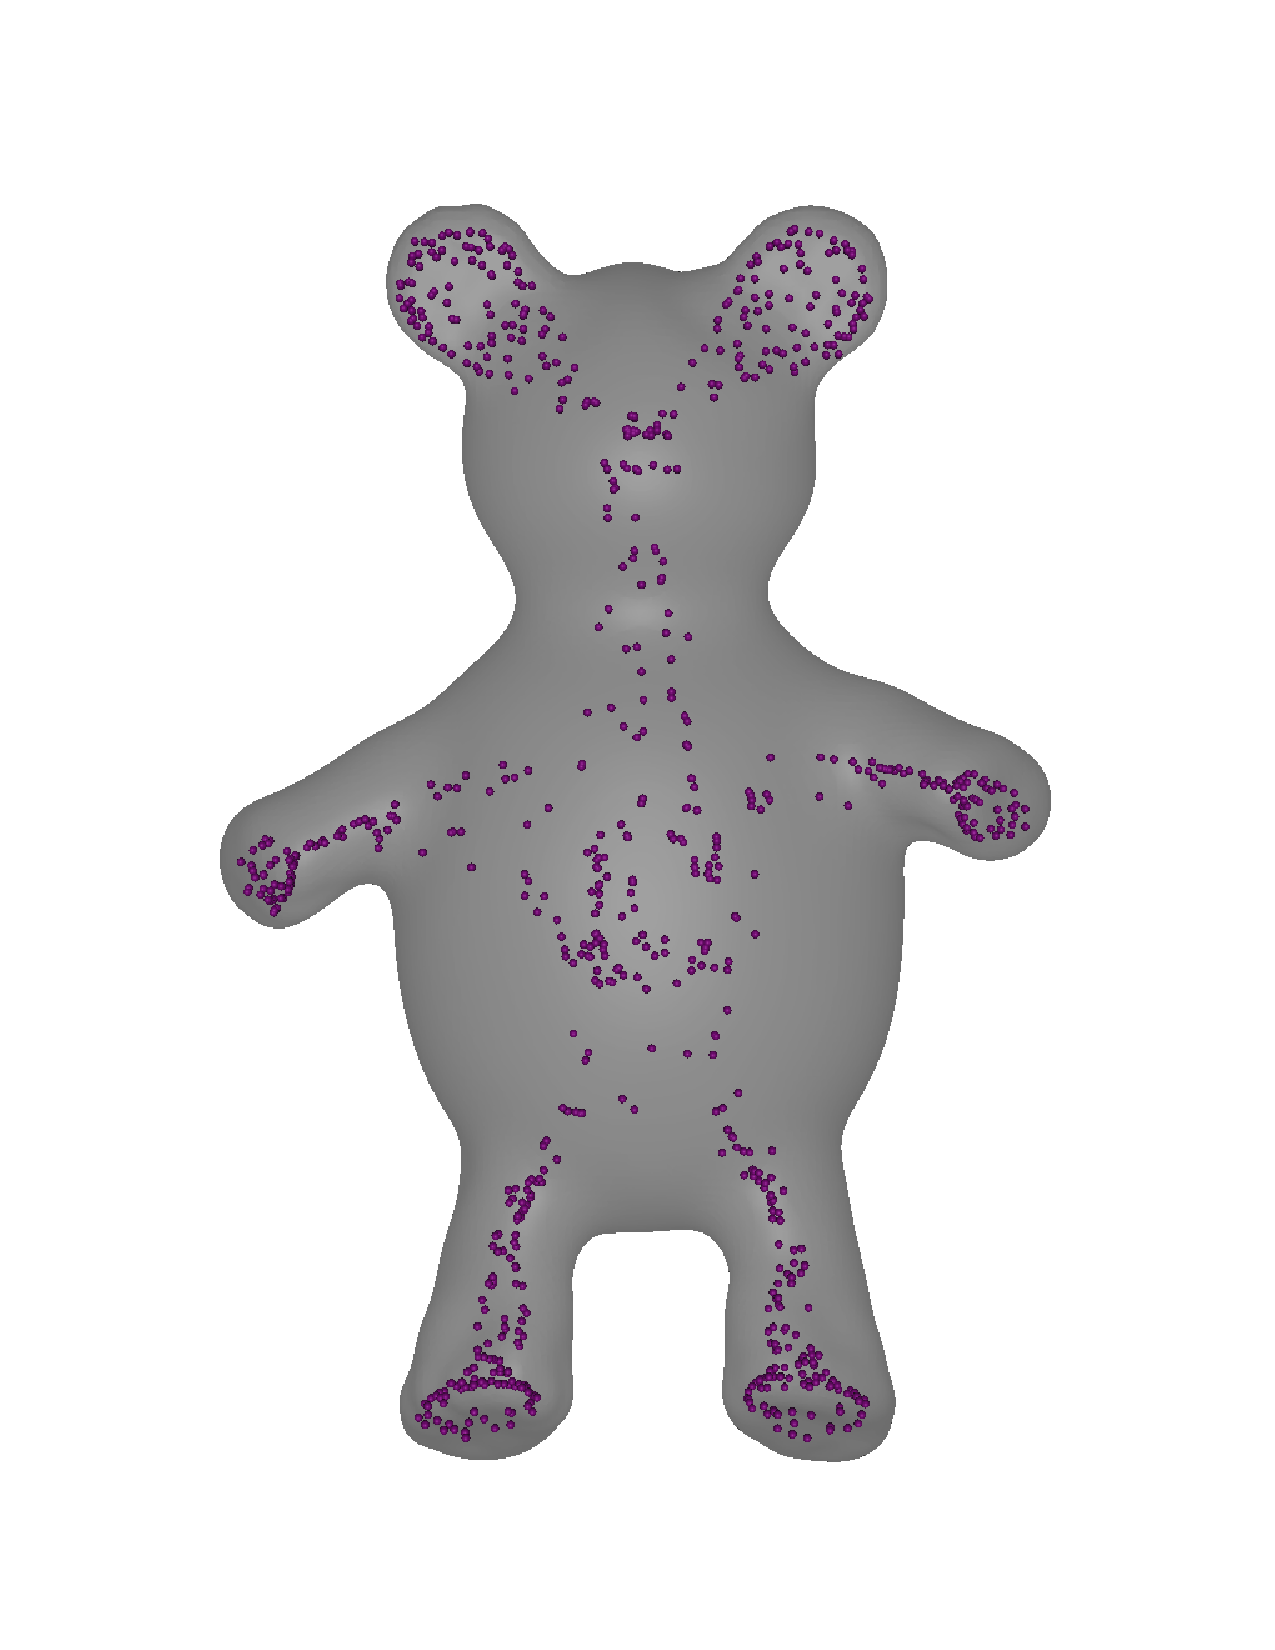
\includegraphics[width=\textwidth]{images/bear/3.pdf}
        \end{subfigure}
~
		\begin{subfigure}[b]{0.19\linewidth}
                \centering
                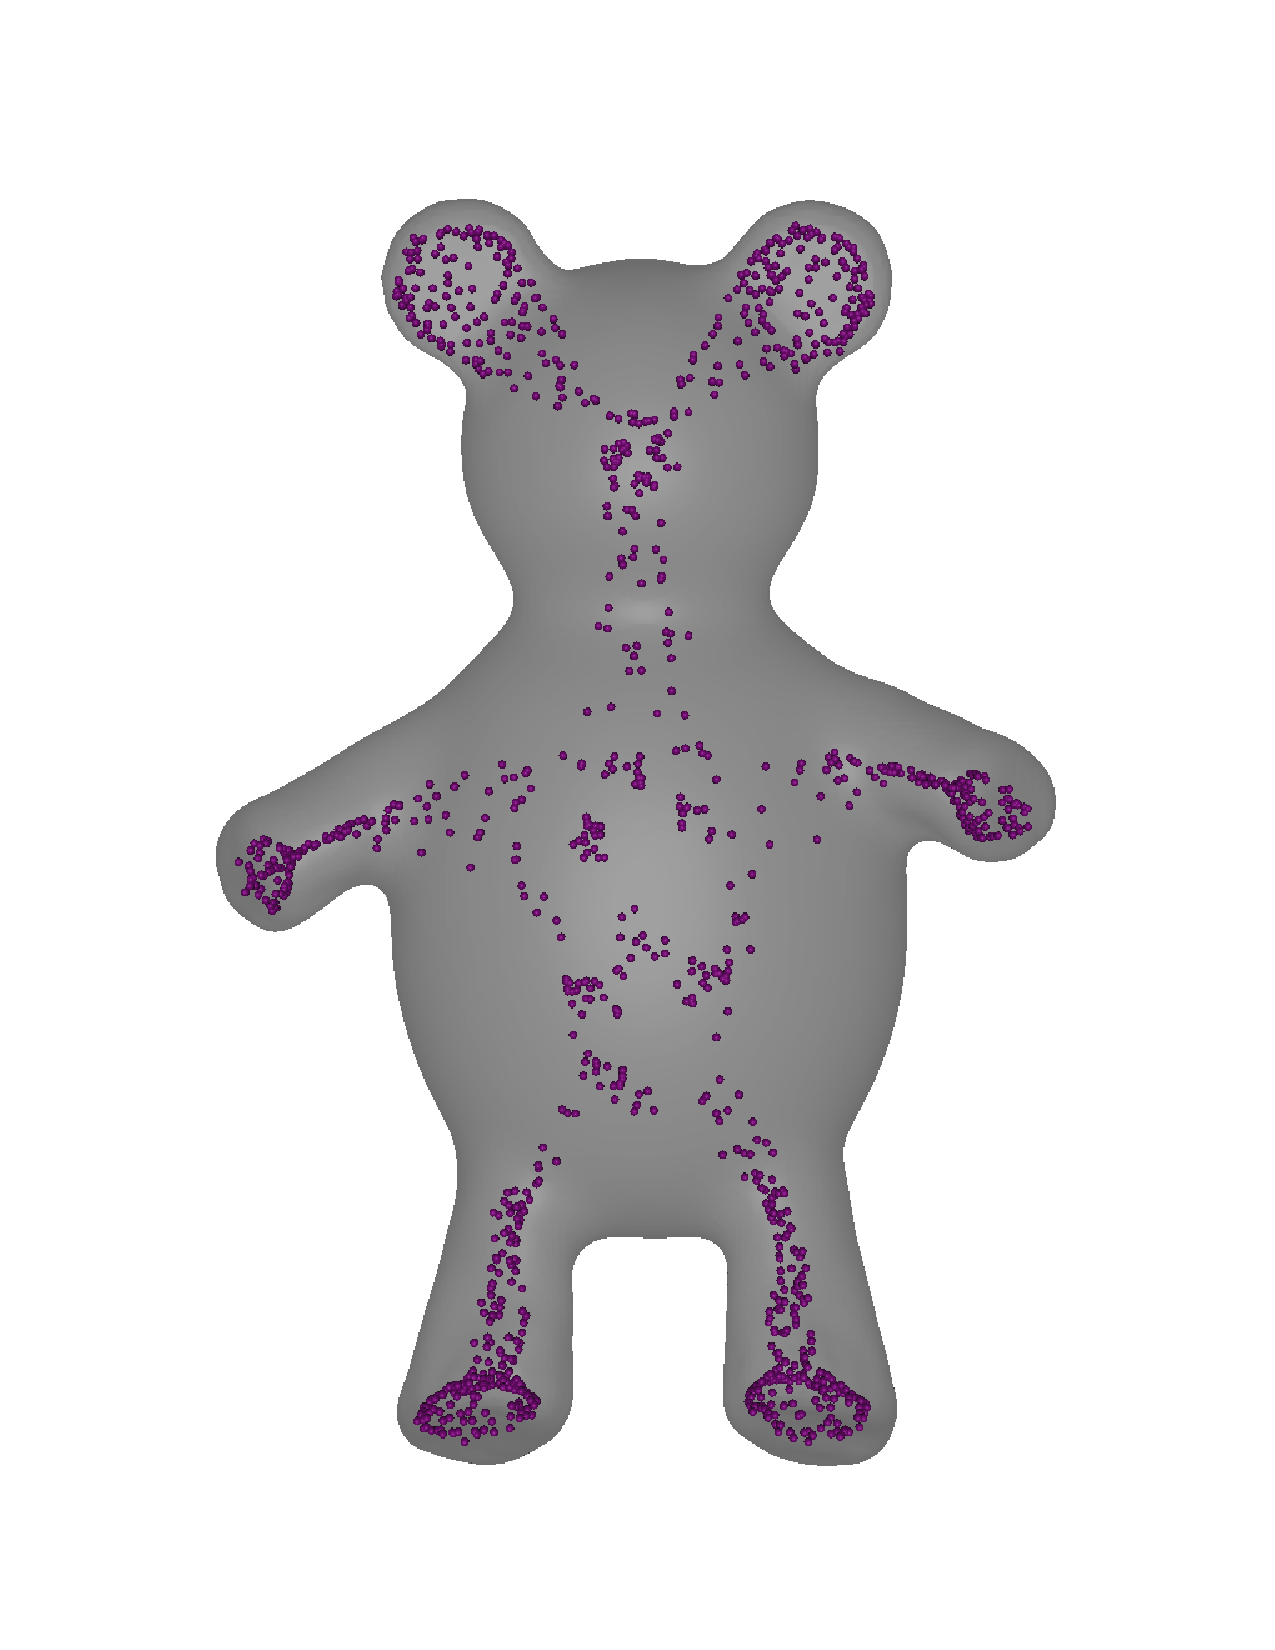
\includegraphics[width=\textwidth]{images/bear/4.pdf}
        \end{subfigure}
        \caption{Chinese calligraphy which means 'horse'. From left to right: ground truth, shape of the signed distance field approximated by the radial basis function, signed distance field at height = $0.025$, $0.05$ and $0.075$, respectively. }
				\label{fig:horse}
\end{figure*}



\textbf{Sparsity comparing with former approaches. }


\textbf{Distance Field Building. } 
As we discussed, our aim of optimization is to build the distance field inside the shape, while keeping the radial basis function value lower than 0 outside the shape. The error between radial basis function and distance field at medial axis points are regularized with constraint []. By setting $\epsilon_2$ in the constraint to a small value, we could get high quality distance field within the shape after the optimization process. Figure~\ref{fig:horse} shows the distance field reconstructed on a Chinese character 'horse', with $\epsilon_2=0.05$. Note that previous methods like Possion or MPU could only construct reliable distance field near the data points, not in the whole inner space of the shape. Our method, on the other hand, could retrieve distance field deep in shape. The 3 subfigures in Figure~\ref{fig:horse} shows am application of the signed distnace field we've obtained: We could offset the Chinese character easily by extracting isocurves of different heights from the radial basis fucntion.
\begin{figure*}
        \centering
		\begin{subfigure}[b]{0.16\linewidth}
                \centering
                
\includegraphics[width=\textwidth]{images/horse/horse.pdf}
        \end{subfigure}
        ~
		\begin{subfigure}[b]{0.18\linewidth}
                \centering
                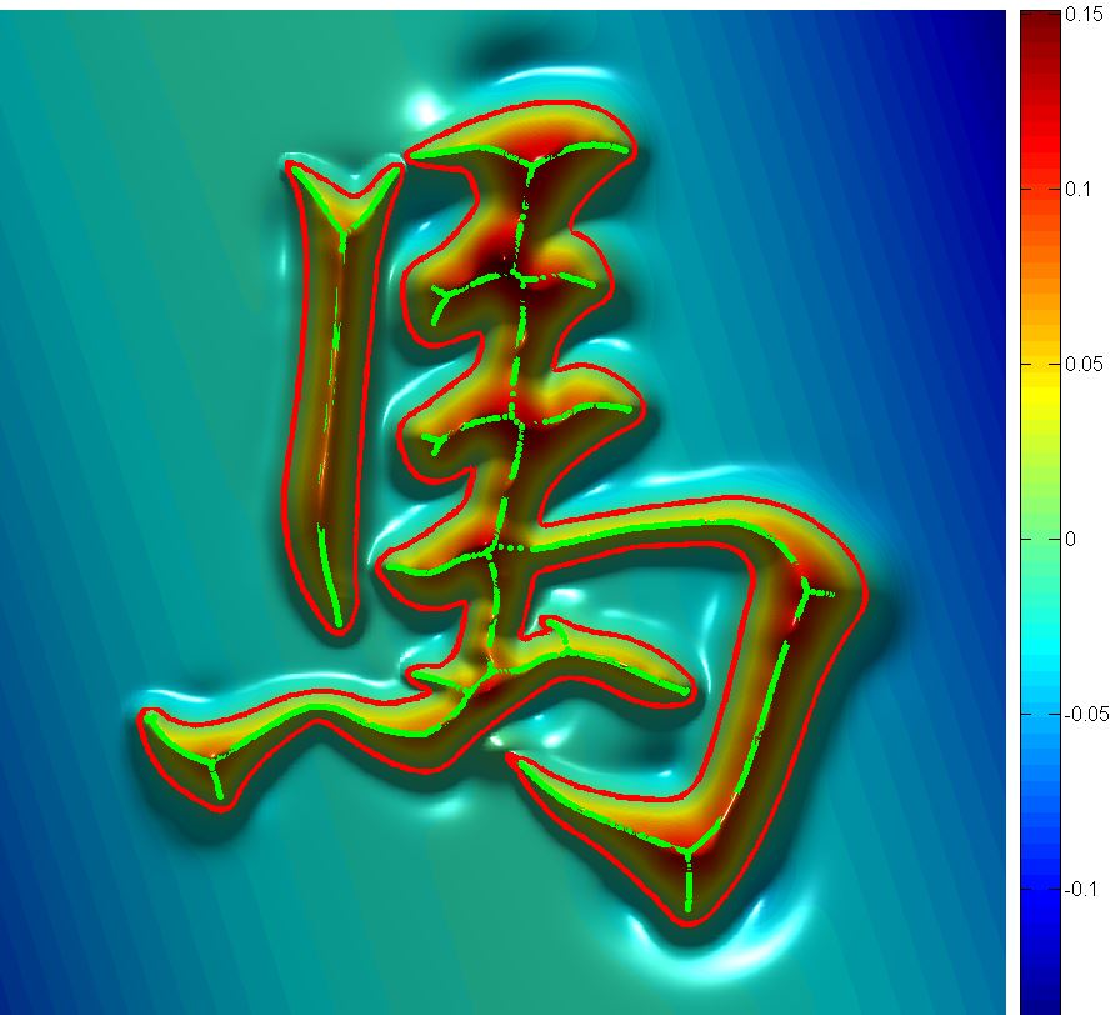
\includegraphics[width=\textwidth]{images/horse/horse_3d.pdf}
        \end{subfigure}
        ~
		\begin{subfigure}[b]{0.18\linewidth}
                \centering
                
\includegraphics[width=\textwidth]{images/horse/horse-contour-0d25.pdf}
        \end{subfigure}
		~
		\begin{subfigure}[b]{0.18\linewidth}
                \centering
                
\includegraphics[width=\textwidth]{images/horse/horse-contour-0d5.pdf}
        \end{subfigure}
~
		\begin{subfigure}[b]{0.18\linewidth}
                \centering
                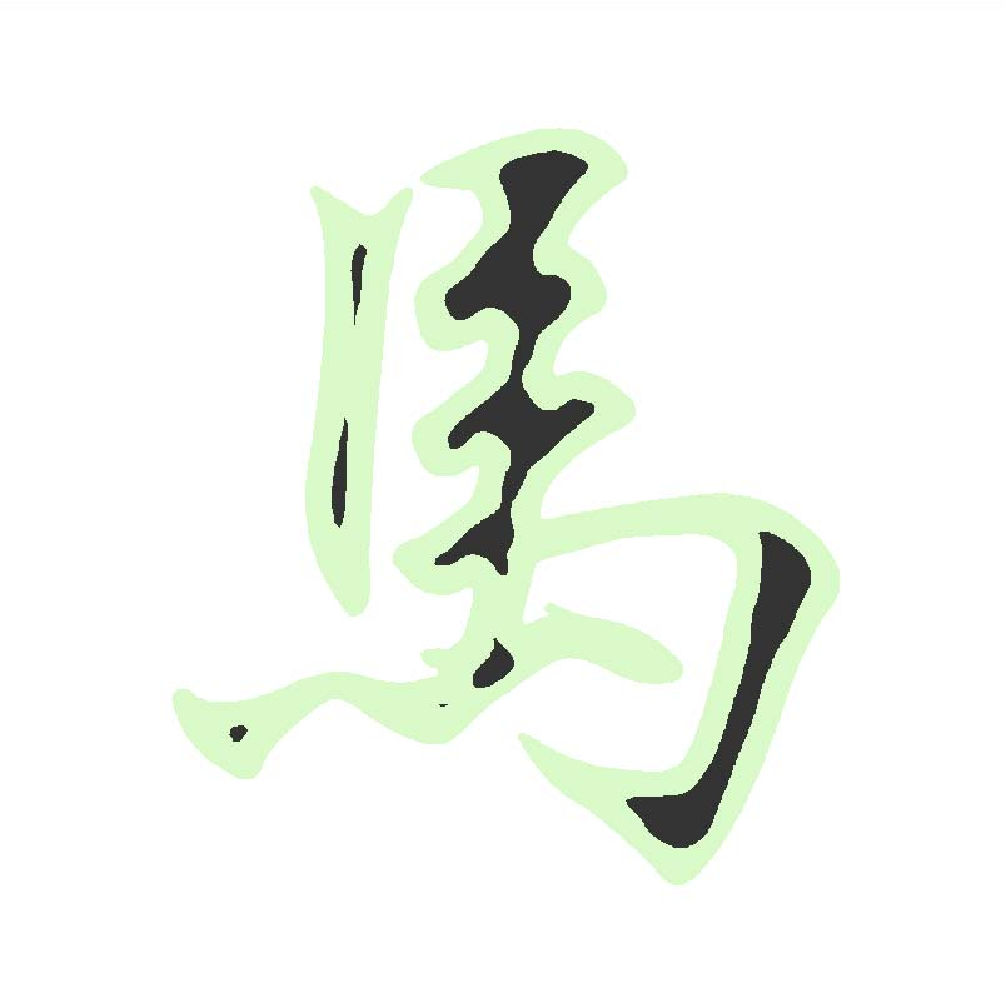
\includegraphics[width=\textwidth]{images/horse/horse-contour-0d75.pdf}
        \end{subfigure}
        \caption{Chinese calligraphy which means 'horse'. From left to right: ground truth, shape of the signed distance field approximated by the radial basis function, signed distance field at height = $0.025$, $0.05$ and $0.075$, respectively. }
				\label{fig:horse}
\end{figure*}

\textbf{Distance Field vs Sparsity. }
Readers may notice that the ridge anchor constraints [], which is measured by $L^{\infty}$-norm, impose constraints on each anchor points. This is seemingly an obstacle to the final sparsity in solution. Figure [] surveyed the relation among the selection of $\epsilon_2$, the reconstruction error, and the sparsity. 

\textbf{Multiscale shape represnetation abilitiy. } 
Many real world shapes contain both bulky and tiny parts. To reconstruct these shapes, local or hierarchical methods need to carefully detect the variation of scales and to properly re-scale in order to match the local level of detail. Our method, on the other hand, uses radial basis which radius are porportional to the scale of the shape. Then, the constraints [] used to build signed distance field are set as relative error constraints to cope with the difference in shape scale. As a result, our method actually transforms a multi-scale input shape to a uniform-scale signed distance field reconstruction problem. In this sense, we do not need to take any additional care on relatively tiny parts of the shape. Figure ?? shows the radial basis function representation and signed distance field representing the shape of a rhenoceros. Note how the thin tail and bulky body of the rhenoceros are reconstructed simultaneously when we built the signed distance field. Figure ?? shows the shape of a seahorse with many spikes on its body reconstructed by our method. Geometric details near each spike are reconstructed by a sequence of radial basis' approaching the spike with diminishing radius. 

\begin{figure}
        \centering
		\begin{subfigure}[b]{0.34\linewidth}
                \centering
                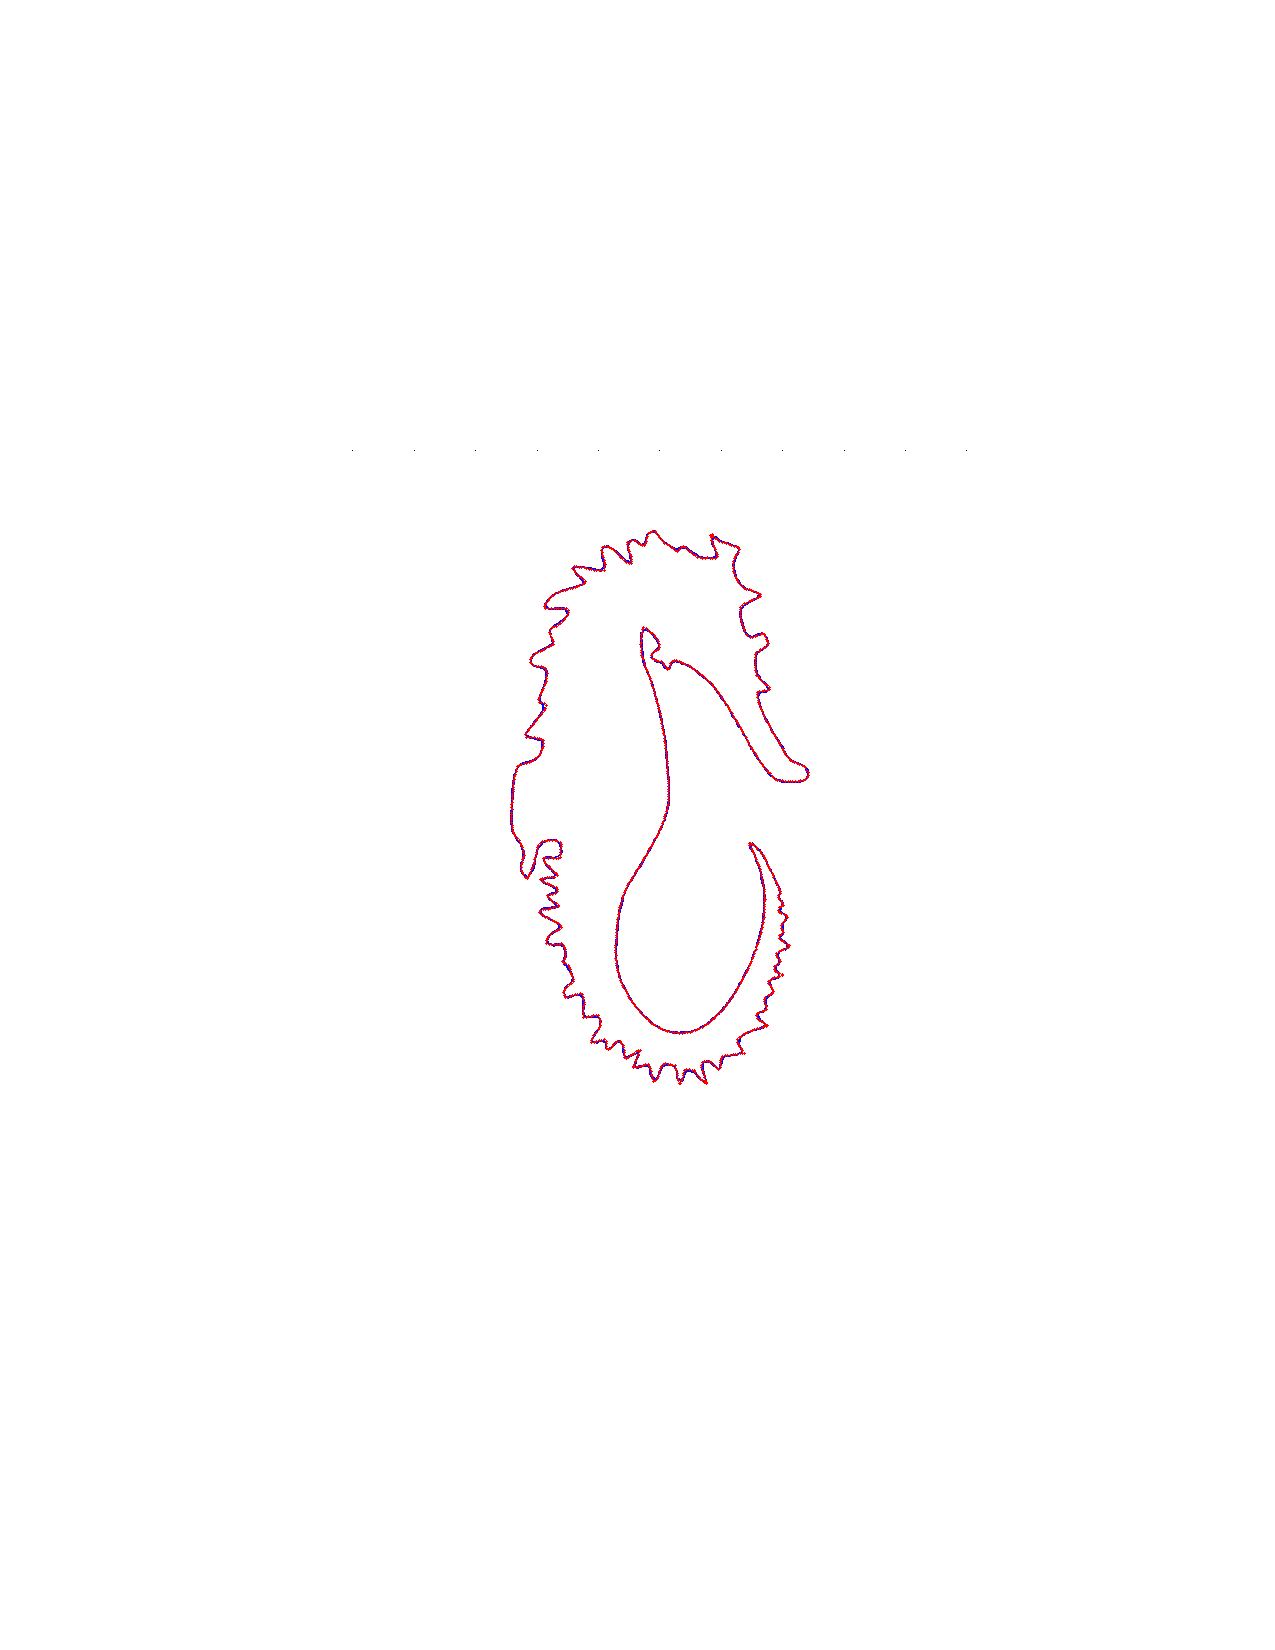
\includegraphics[width=\textwidth]{images/seahorse/1.pdf}
       \end{subfigure}
		~
		\begin{subfigure}[b]{0.34\linewidth}
                \centering
                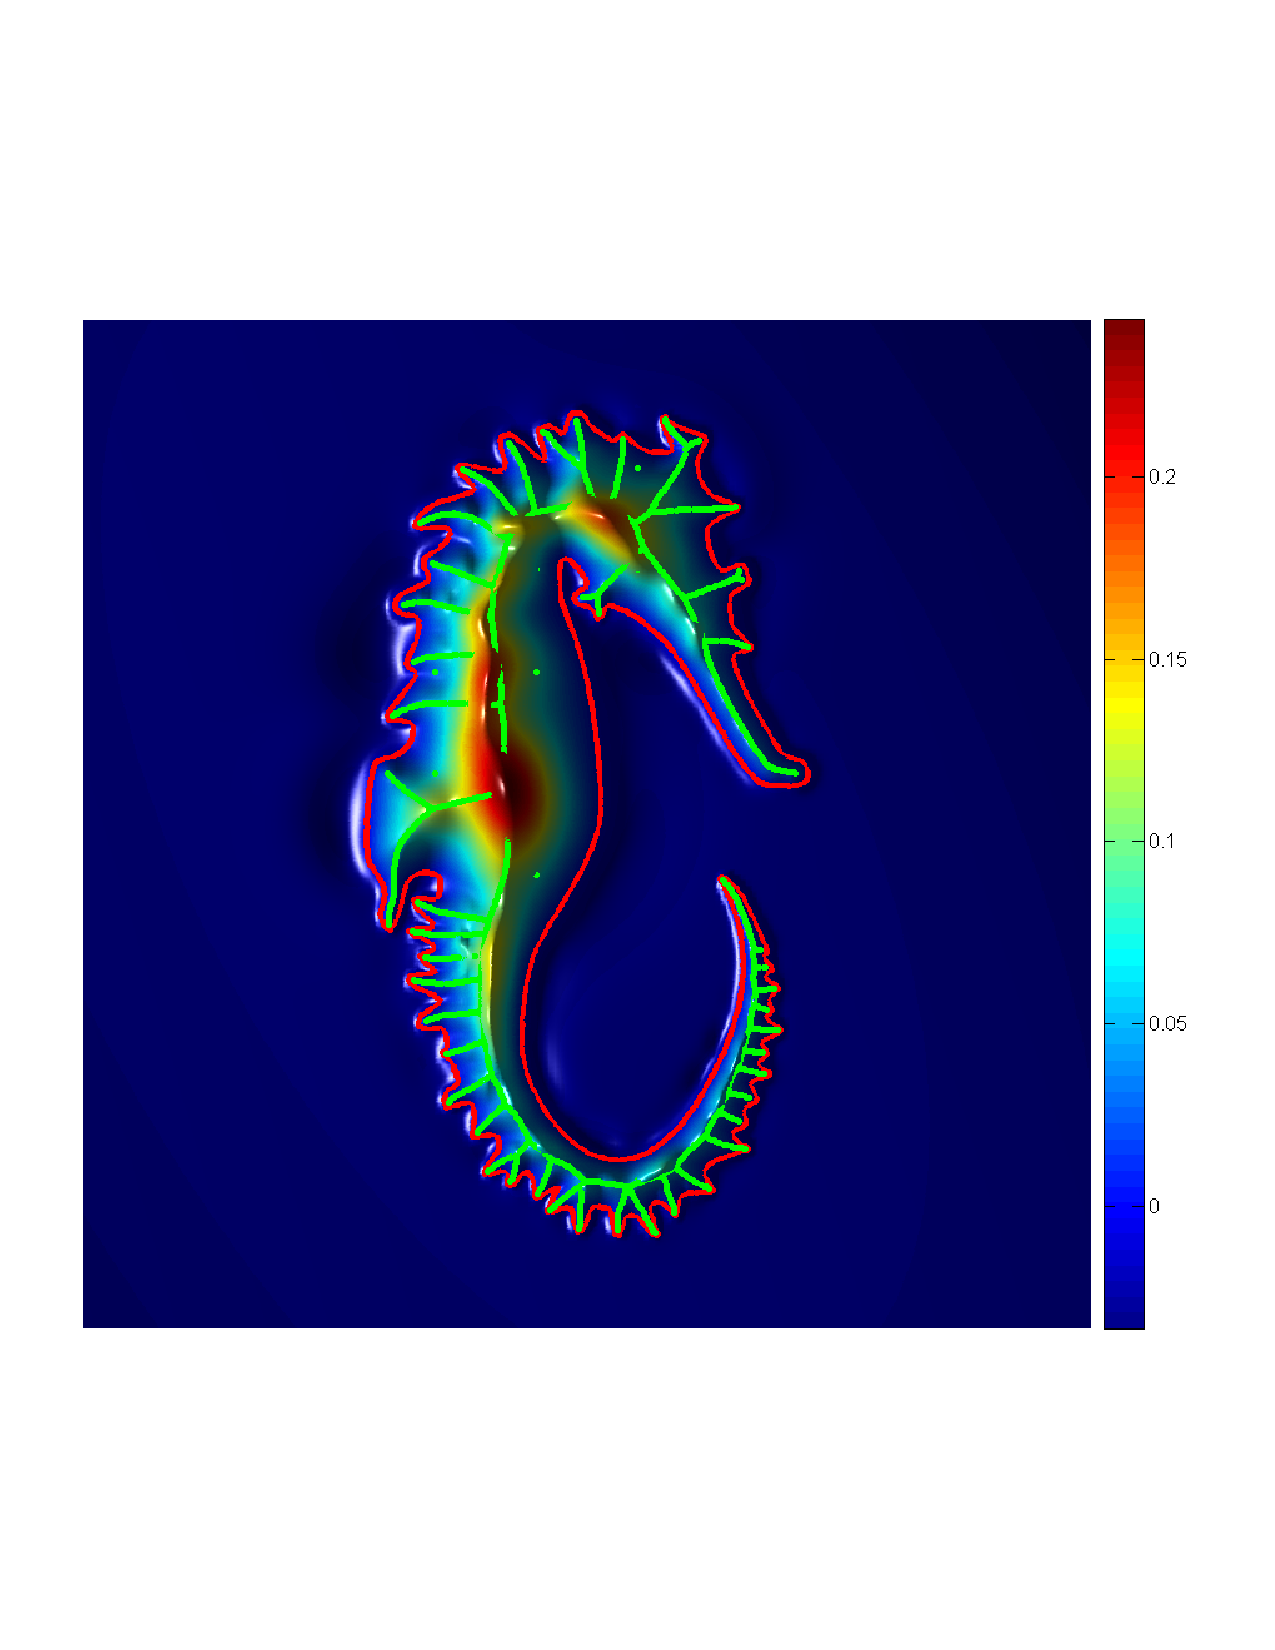
\includegraphics[width=\textwidth]{images/seahorse/2.pdf}
        \end{subfigure}
~
		\begin{subfigure}[b]{0.25\linewidth}
                \centering
                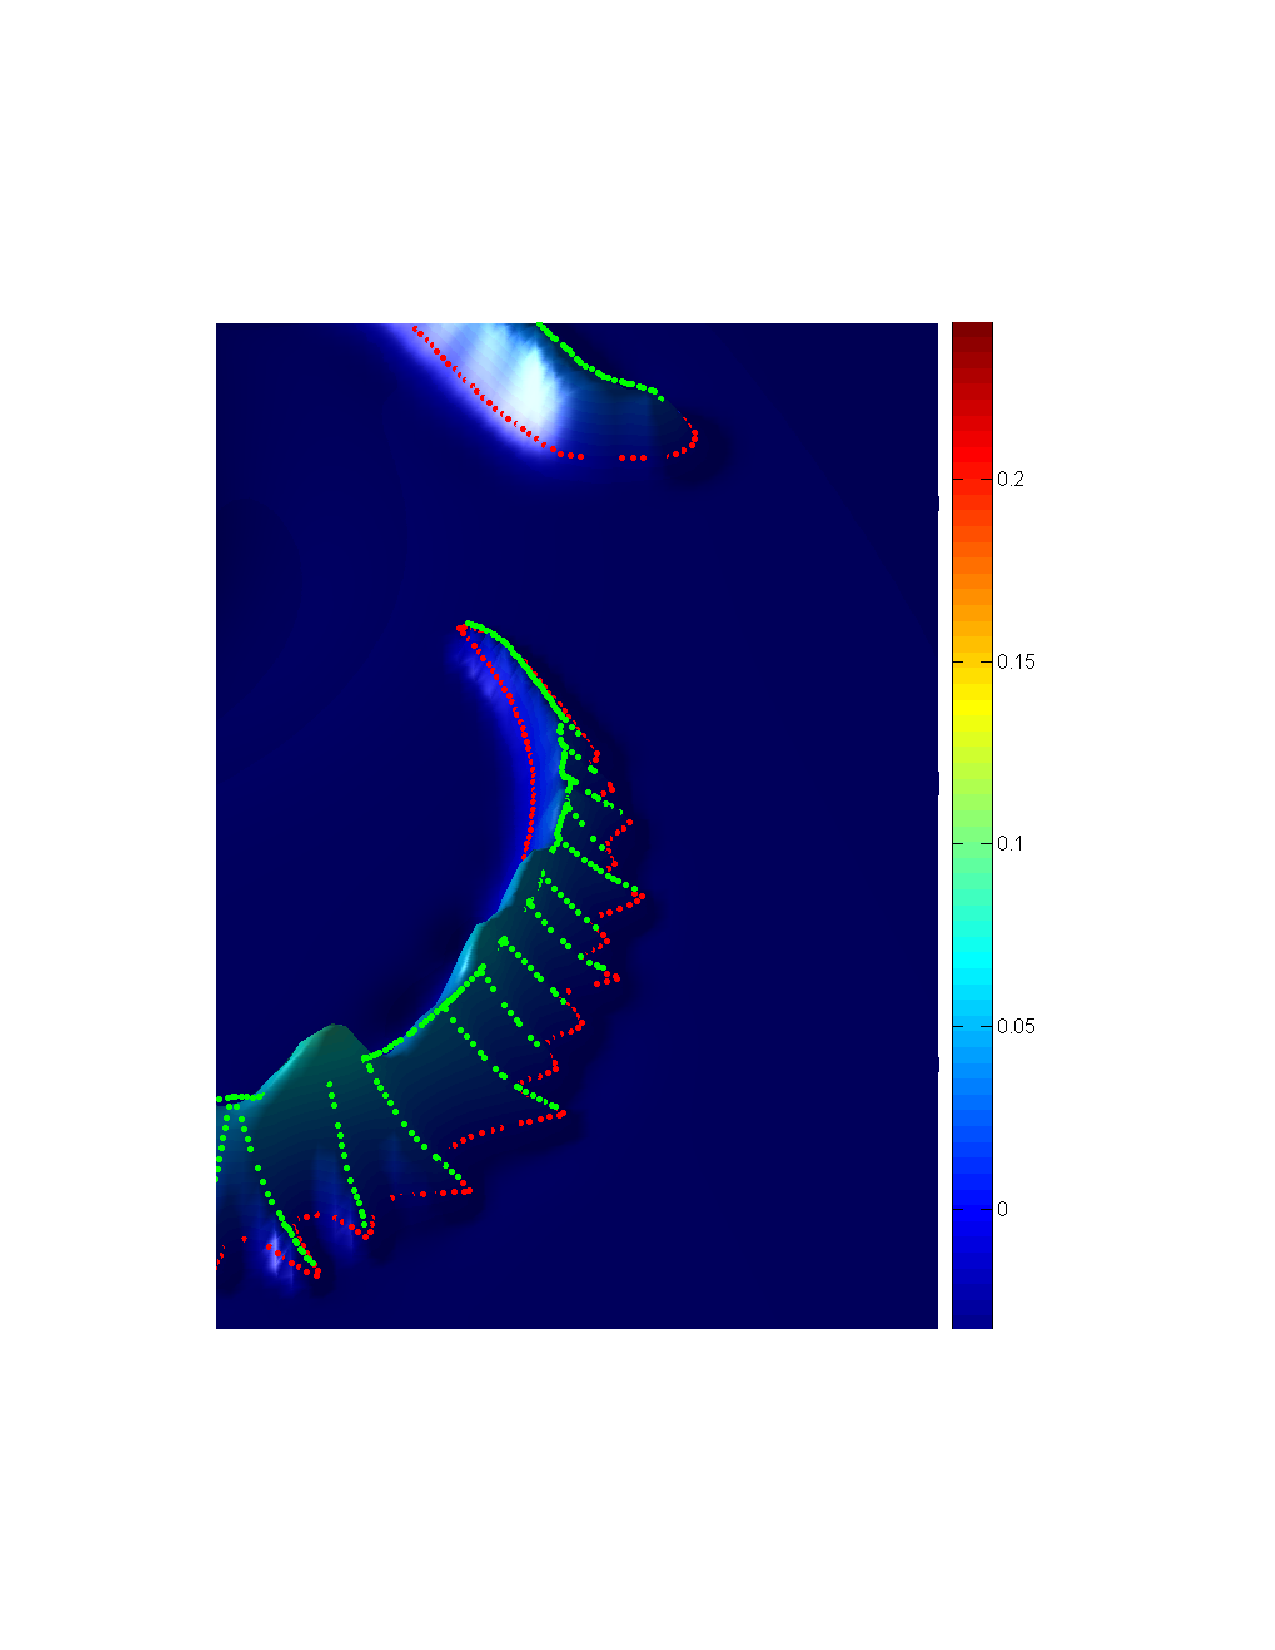
\includegraphics[width=\textwidth]{images/seahorse/3.pdf}
        \end{subfigure}
        \caption{Chinese calligraphy which means 'horse'. From left to right: ground truth, shape of the signed distance field approximated by the radial basis function, signed distance field at height = $0.025$, $0.05$ and $0.075$, respectively. }
				\label{fig:horse}
\end{figure}

\begin{figure}
        \centering
		\begin{subfigure}[b]{0.3\linewidth}
                \centering
                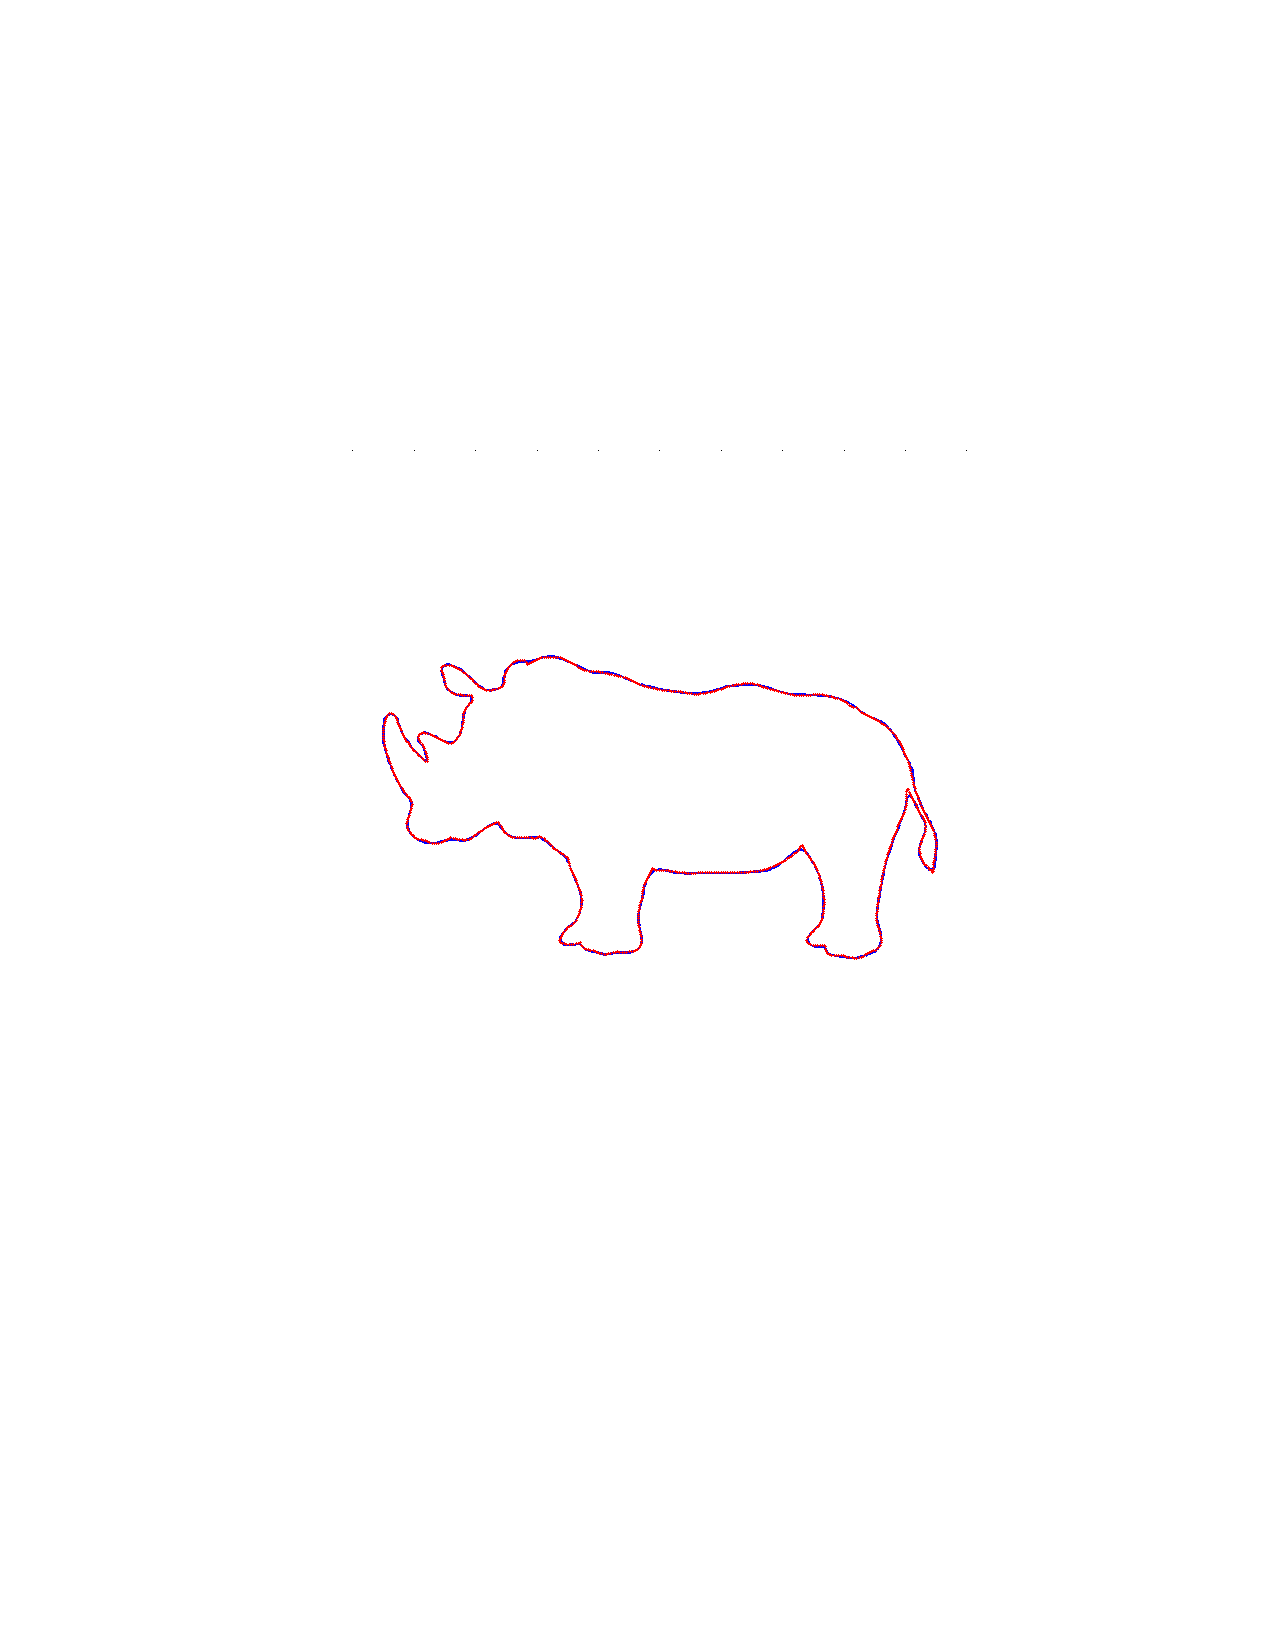
\includegraphics[width=\textwidth]{images/rhenoceros/1.pdf}
       \end{subfigure}
		~
		\begin{subfigure}[b]{0.33\linewidth}
                \centering
                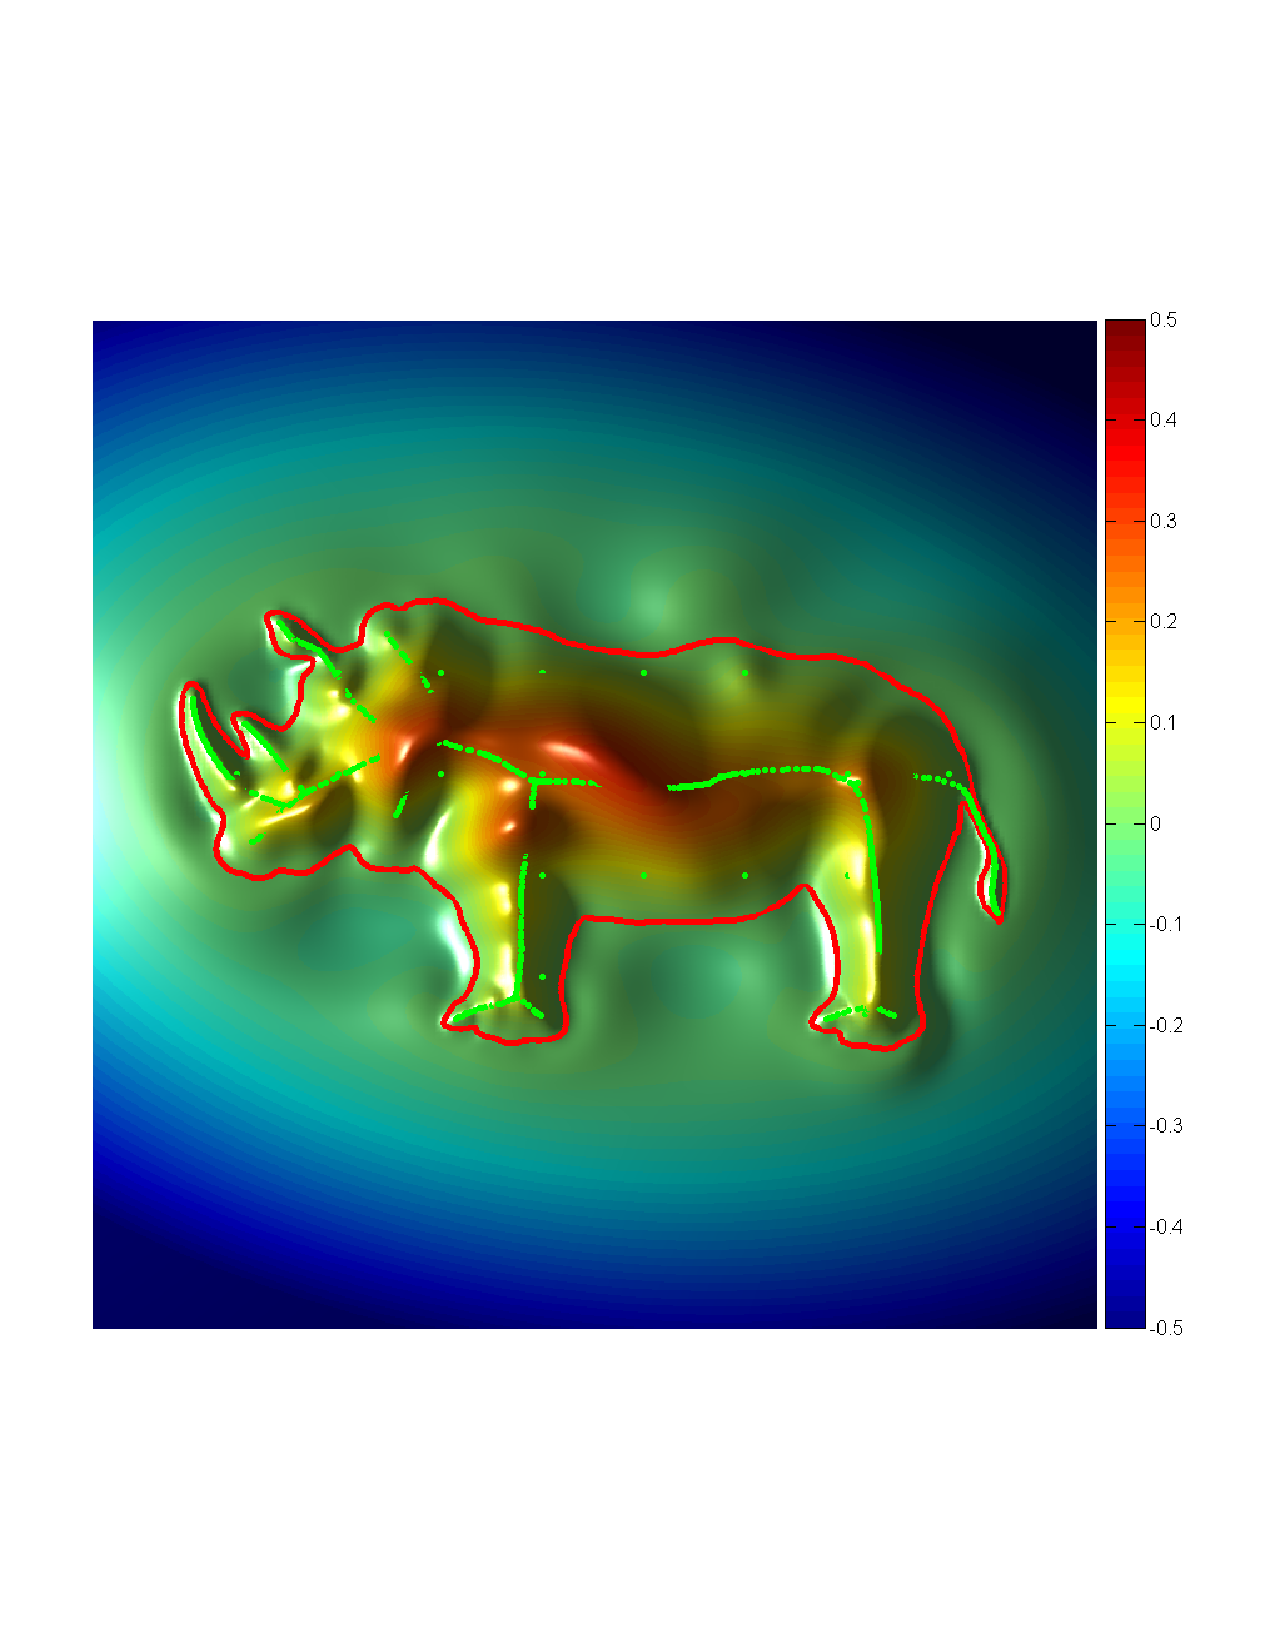
\includegraphics[width=\textwidth]{images/rhenoceros/2.pdf}
        \end{subfigure}
~
		\begin{subfigure}[b]{0.3\linewidth}
                \centering
                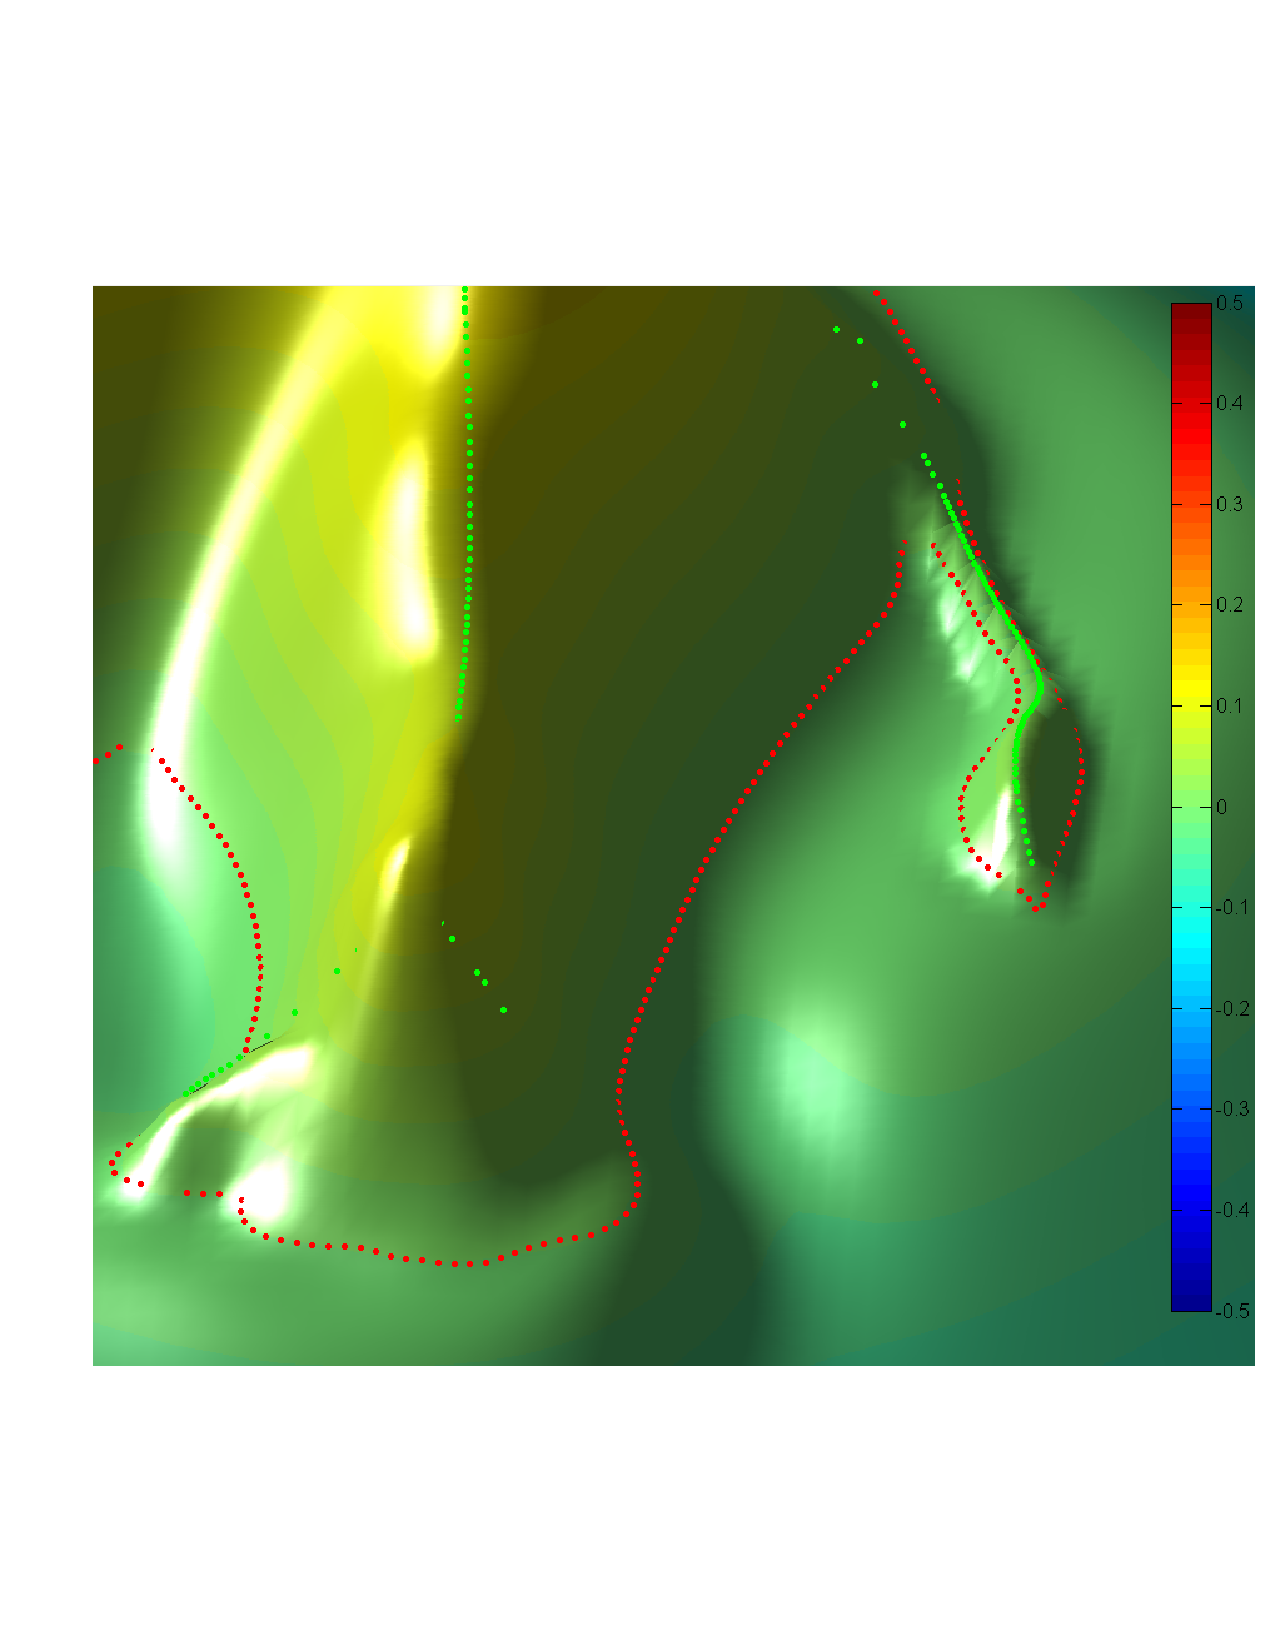
\includegraphics[width=\textwidth]{images/rhenoceros/3.pdf}
        \end{subfigure}
        \caption{Chinese calligraphy which means 'horse'. From left to right: ground truth, shape of the signed distance field approximated by the radial basis function, signed distance field at height = $0.025$, $0.05$ and $0.075$, respectively. }
				\label{fig:horse}
\end{figure}


\textbf{Robustness to Point Normal Noise. }
Implicit reconstruction methods such as MPU and Poisson need accurate normal infomation associated with input data points for a high quality output. These methods are known to be prone to noise in normal information []. On the other hand, computing surface normal is not a trifle problem especially for shapes containing sharp features or of complicated topology structure. Medial axis computation does not need point normal as prerequisite, so our method could better adapt to problems in which normals could not be confidentally computed. Figure ?? shows an example of a thick knot. In this example, some surfaces closing to each other in terms of Euclidean are far away from each other in the sense of geodesic distance. Computation of surface normal in this example is not easy, but this difficulty will not effect our method.

\section{Limitation and Future Work}
Unlike local and hierarchical methods, our method considers the full point cloud as well as the complete medial axis(after simple filtering) as a whole. These two sets of points will form a large matrix in optimization. Furthermore, as the radius $r_i$ of radial basis are not uniform but set as the radius of medial axis spheres, local support area of different radial basis also differ from one to another, causing the sparsity pattern of the matrix to be irregular. Therefore, measured by computing speed, our method is slower than MPU and Poisson method as a method for surface reconstruction. Another issue is the memory needed to store the matrix used in computation. Gaussian function is not sparse but degenerates quickly as radius increases. In practice, if we cut-off the Gaussian function at 4-$\sigma$ position(where the value of radial basis is $1.1\times 10^{-7})$, then we could obtain a matrix with approximately $95\%$ zero elements, and in this case we could handle problem with about 40,000 data points and 30,000 medial axis points on a PC with 16GB RAM. However, we could not handle some very complicated examples which more data points / medial axis points than this limit. 

[FUTURE WORK HERE]

\section*{Acknowledgements}

\section*{Appendix: ADMM Solver for the Convex Optimization Problem}
We follow the common notation in ADMM. The variables subject to $L^1$-norm minimization is denoted as $x$ (in our problem, $x=(c_1,...c_n)$ ). The pointwise $L^2$-error constraints(Eqn.~\ref{eq:2}), ridge anchor constraints(Eqn.~\ref{eq:3}) and sign anchor constraints(Eqn.~\ref{eq:4}) could be written in matrix form, along with the $L^1$-norm minimization(Eqn.~\ref{eq:1}), as:
\begin{align}
&\min\|x\|_1\\
\mbox{s.t.: }&\|Ax-b\|_2^2<\epsilon_1\sqrt{N},\\
&\|Cx-d\|_{\infty}<\epsilon_2,\\
&[Mx-v]_i<\epsilon_3,\quad\forall i.
\end{align}
Where $A_{ij}=B_j(\mathbf{X}_i)$ is the value of the $j$-th radial basis at $\mathbf{X}_i$. $b$ is a 0-vector as we choose the isosurface at height 0 to approximate the input shape. $C_{ij}=B_j(\mathbf{M}_i)$ is the value of the $j$-th radial basis at the medial sphere center $\mathbf{M}_i$, scaled by the diagonal matrix $D$ Eqn.~\ref{eq:3}. $d$, after scaling by $D$ in Eqn.~\ref{eq:3}, is an all-one vector. $M_{ij}=B_j(\mathbf{G}_i)$ is the value of the $j$-th radial basis on the sign anchor $G_i$, and $v$ is a 0-vector in our optimization.

For ADMM, this equivant to:
\begin{align}
&\min\|x\|_1\\
\mbox{s.t. }&y_1-x=0,\\
&Ay_1-b-y_2=0,\\
&Cy_1-d-y_3=0,\\
&My_1-v-y_4=0,\\
&\|y_2\|_2<\epsilon_1\sqrt{N},\\
&\|y_3\|_{\infty}<\epsilon_2,\\
&y_4<\epsilon_3.
\end{align}
The Lagrangian for the above equation array is:
\begin{align}
L_\rho=&\|x\|_1+\frac{\rho_1}{2}\|y_1-x+u_1\|^2\notag\\
&+\frac{\rho_2}{2}\|Ay_1-b-y_2+u_2\|^2+\frac{\rho_3}{2}\|Cy_1-d-y_3+u_3\|^2\notag\\
&+\frac{\rho_4}{2}\|My_1-v-y_4+u_4\|^2+\Pi_{\{\|\cdot\|_2<\epsilon_1\}}(y_2)\notag\\
&+\Pi_{\{\|\cdot\|_{\infty}<\epsilon_2\}}(y_3)+\Pi_{\{[\cdot]_i<\epsilon_3\}}(y_4).
\end{align}
In which $\Pi_{\mathcal{C}}(\cdot)$ is the indicator function defined on set $\mathcal{C}$.

Now we could write down ADMM steps to update each variable: 
\begin{align}
y_1^{k+1}=&\operatornamewithlimits{argmin}\limits_{y_1} \Big\{\frac{\rho_1}{2}\|y_1-x^k+u_1^k\|^2\notag\\
&+\frac{\rho_2}{2}\|Ay_1-b-y_2^k+u_2^k\|^2\notag\\
&+\frac{\rho_3}{2}\|Cy_1-d-y_3^k+u_3^k\|^2\notag\\
&+\frac{\rho_4}{2}\|My_1-v-y_4^k+u_4^k\|^2 \Big\} \\
x^{k+1}=&\operatornamewithlimits{argmin}\limits_{x} \Big\{\|x\|_1+\frac{\rho_1}{2}\|y_1^{k+1}-x+u_1^k\|^2\Big\}\\
y_2^{k+1}=&\operatornamewithlimits{argmin}\limits_{y_2} \Big\{\frac{\rho_2}{2}\|Ay_1^{k+1}-b-y_2+u_2^k\|^2\notag\\&+\Pi_{\{\|\cdot\|_2<\epsilon_1\}}(y_2)\Big\}\\
y_3^{k+1}=&\operatornamewithlimits{argmin}\limits_{y_3} \Big\{\frac{\rho_3}{2}\|Cy_1^{k+1}-d-y_3+u_3^k\|^2\notag\\&+\Pi_{\{\|\cdot\|_{\infty}<\epsilon_2\}}(y_3)\Big\}\\
y_4^{k+1}=&\operatornamewithlimits{argmin}\limits_{y_4} \Big\{\frac{\rho_4}{2}\|My_1^{k+1}-v-y_4+u_4^k\|^2\notag\\&+\Pi_{\{[\cdot]_i<\epsilon_3\}}(y_4)\Big\}\\
u_1^{k+1}=&u_1^k+\gamma(y_1^{k+1}-x^{k+1})\\
u_2^{k+1}=&u_2^k+\gamma(Ay_1^{k+1}-b-y_2^{k+1})\\
u_3^{k+1}=&u_3^k+\gamma(Cy_1^{k+1}-d-y_3^{k+1})\\
u_4^{k+1}=&u_4^k+\gamma(My_1^{k+1}-v-y_4^{k+1})\\
\end{align}
To solve it:
\begin{align}
y_1^{k+1}=&\Big( \rho_1 I+ \rho_2 A^TA+ \rho_3 C^TC+ \rho_4 M^TM\Big)^{-1}\cdot\notag\\
&\cdot\Big(\rho_1 (x^k-u_1^k)+\rho_2 A^T(b+y_2^k-u_2^k)\notag\\ &+ \rho_3 C^T(d+y_3^k-u_3^k)+\rho_4 M^T(v+y_4^k-u_4^k)\Big)\\
x_1^{k+1}=&\max\Big(y_1^{k+1}+u_1^k-\frac{1}{\rho_1}, 0\Big) \notag\\&- \max\Big(-y_1^{k+1}-u_1^k-\frac{1}{\rho_1}, 0\Big)\\
y_2^{k+1}=&\min\Big(\frac{\epsilon_1}{\|Ay_1^{k+1}+u_2^k-b\|},1\Big)\cdot\big(Ay_1^{k+1}+u_2^k-b\big)\\
y_{3,i}^{k+1}=&\left\{
\begin{array}{ll}
(Cy_1^{k+1}+u_3^k-d)_i, &\mbox{if }|(Cy_1^{k+1}+u_3^k-d)_i|\leq\epsilon_2,\\
\epsilon_2, &\mbox{if }(Cy_1^{k+1}+u_3^k-d)_i>\epsilon_2,\\
-\epsilon_2, &\mbox{if }(Cy_1^{k+1}+u_3^k-d)_i<-\epsilon_2.\\
\end{array}
\right.\\
y_{4,i}^{k+1}=&\left\{
\begin{array}{ll}
(My_1^{k+1}+u_4^k-v)_i, &\mbox{if }(My_1^{k+1}+u_4^k-v)\leq\epsilon_3,\\
\epsilon_3, &\mbox{if }(My_1^{k+1}+u_4^k-v)>\epsilon_3,\\
\end{array}
\right.\\
u_1^{k+1}=&u_1^k+\gamma(y_1^{k+1}-x^{k+1})\\
u_2^{k+1}=&u_2^k+\gamma(Ay_1^{k+1}-b-y_2^{k+1})\\
u_3^{k+1}=&u_3^k+\gamma(Cy_1^{k+1}-d-y_3^{k+1})\\
u_4^{k+1}=&u_4^k+\gamma(My_1^{k+1}-v-y_4^{k+1})
\end{align}
$\gamma$ is a relaxation term used to improve convergence. We fix $\gamma=1.6$ during the process of optimization in this paper. 

As the constrained convex optimization problem has unique local minimum, different choice of initial values will hardly affect the optimization result. We set all variables $x, y_1, y_2, y_3, y_4, u_1, u_2, u_3$ and $u_4$ as 0 when optimization started. 

Some literatures, such as [] [] and [] discussed the strategy to vary parameters $\{\rho_i\}$ during the process of optimization for acceleration. Nevertheless, convergence of ADMM is no longer guaranteed supposing $\{\rho_i\}$ are not fixed during iterations. Additionally, in our problem, upon the change of $\{\rho_i\}$, matrix $P$ used for $y_1$ update in ADMM must be calculated and decomposed again, causing considerable computational overhead. Thereore, in our approach, we fix $\{\rho_i\}$ as $\rho_1=1000, \rho_2=1000, \rho_3=1, \rho_4=50$ as an emperical parameter set. These parameters are used for all examples in this paper.
\bibliographystyle{acmsiggraph}
\bibliography{rbf}
\end{document}
